\documentclass[xcolor={dvipsnames,table}]{beamer}
\usecolortheme[named=PineGreen]{structure} 
\usetheme{Warsaw}
\pdfpageattr {/Group << /S /Transparency /I true /CS /DeviceRGB>>}
\usepackage{hyperref}
\usepackage{graphicx}
\usepackage{aas_macros}
\usepackage{array}
\usepackage[utf8x]{inputenc} %So you can say alfvén




\setbeamertemplate{caption}{\raggedright\insertcaption\par}
  \setbeamertemplate{enumerate items}[default]
  \setbeamertemplate{itemize items}{$\sim$}
  
 \expandafter\def\expandafter\insertshorttitle\expandafter{%
 	\insertshorttitle\hfill%
 	\insertframenumber\,/\,\inserttotalframenumber}
  \AtBeginSection[]{
  	\begin{frame}
  		\vfill
  		\centering
  		\begin{beamercolorbox}[sep=18pt,center,shadow=true,rounded=true]{title}
  			\usebeamerfont{title}\secname\par%
  		\end{beamercolorbox}
  		\vfill
  	\end{frame}
  }
  
  \newcommand{\subheader}{    		\begin{center}
  	\begin{beamercolorbox}[sep=4pt,center,shadow=true,rounded=true]{title}
  		\usebeamerfont{title}\subsecname\par%
  	\end{beamercolorbox}
  	\vfill
  	\end{center}}


\newcommand{\req}{\ensuremath{\rho_{eq}}} %Since it's used so often. ensuremath lets it be used in equations or text
\newcommand{\dst}{\ensuremath{D_{st}}} %Now I'm just getting lazy. 
\newcommand{\f}{\ensuremath{F_{10.7}}} %Because latex doesn't allow numbers in commands
\newcolumntype{C}{>{$}c<{$}} %To enable math mode in tables (for saying things like B_z)

\begin{document}
\title[Statistical Modeling of Earth's Plasmasphere]{Statistical Modeling of Earth's Plasmasphere}
\author{Victoir Veibell}
\date{August 25, 2016}
\setbeamertemplate{navigation symbols}{}

\begin{frame}
\titlepage
\end{frame}

\setbeamertemplate{section in toc}{\inserttocsection}
\begin{frame}
	\tableofcontents
\end{frame}

\begin{frame}
	Questions addressed by this dissertation:
	\vfill
	\begin{itemize}
		\item What enhances equatorial plasma mass density (\req) in the plasmatrough? Solar wind (via geomagnetic storms) or internal processes (e.g. ionospheric outflow)?
			\vfill
		\item Does a \req\ enhancement depend on current IMF conditions?
			\vfill
		\item Can a \req\ enhancement be classified or forecasted?
	\end{itemize}
\end{frame}


%%%%%%%%%%%%%%%%%%%%%%%%%%%%%%%%%%%%%%%%%%%%%%%%%%%
%  _____      _                 _            _   _             
% |_   _|    | |               | |          | | (_)            
%   | | _ __ | |_ _ __ ___   __| |_   _  ___| |_ _  ___  _ __  
%   | || '_ \| __| '__/ _ \ / _` | | | |/ __| __| |/ _ \| '_ \ 
%   | || | | | |_| | | (_) | (_| | |_| | (__| |_| | (_) | | | |
%  |___|_| |_|\__|_|  \___/ \__,_|\__,_|\___|\__|_|\___/|_| |_|
%%%%%%%%%%%%%%%%%%%%%%%%%%%%%%%%%%%%%%%%%%%%%%%%%%%
\section{Introduction}

\subsection{System}
\begin{frame} 
	
\begin{figure}[htp]
	\centering
	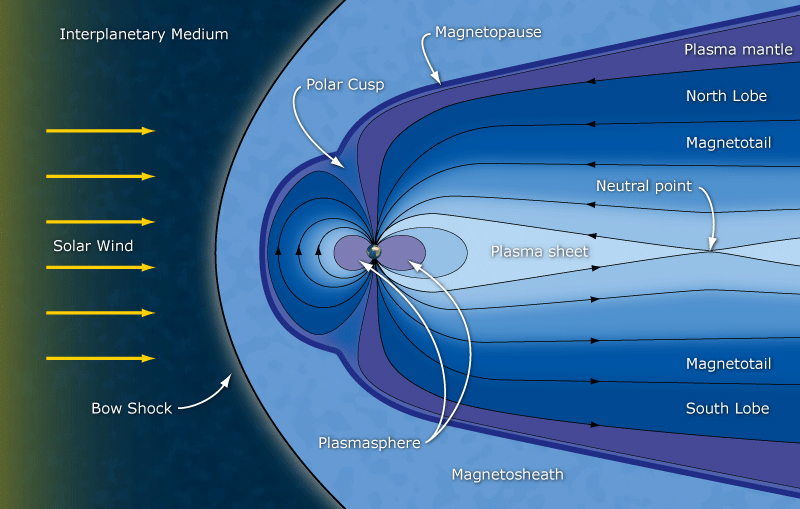
\includegraphics[scale=0.35]{{Figures/MagnetoOverview.jpg}}
	\caption{Overview of the magnetosphere and plasmasphere [Russel (2007)]. Colors used for visual distinctiveness.}
	\label{RingCurrentFigure}
\end{figure}

\end{frame}

\begin{frame}
	\begin{figure}[htp]
		\centering
		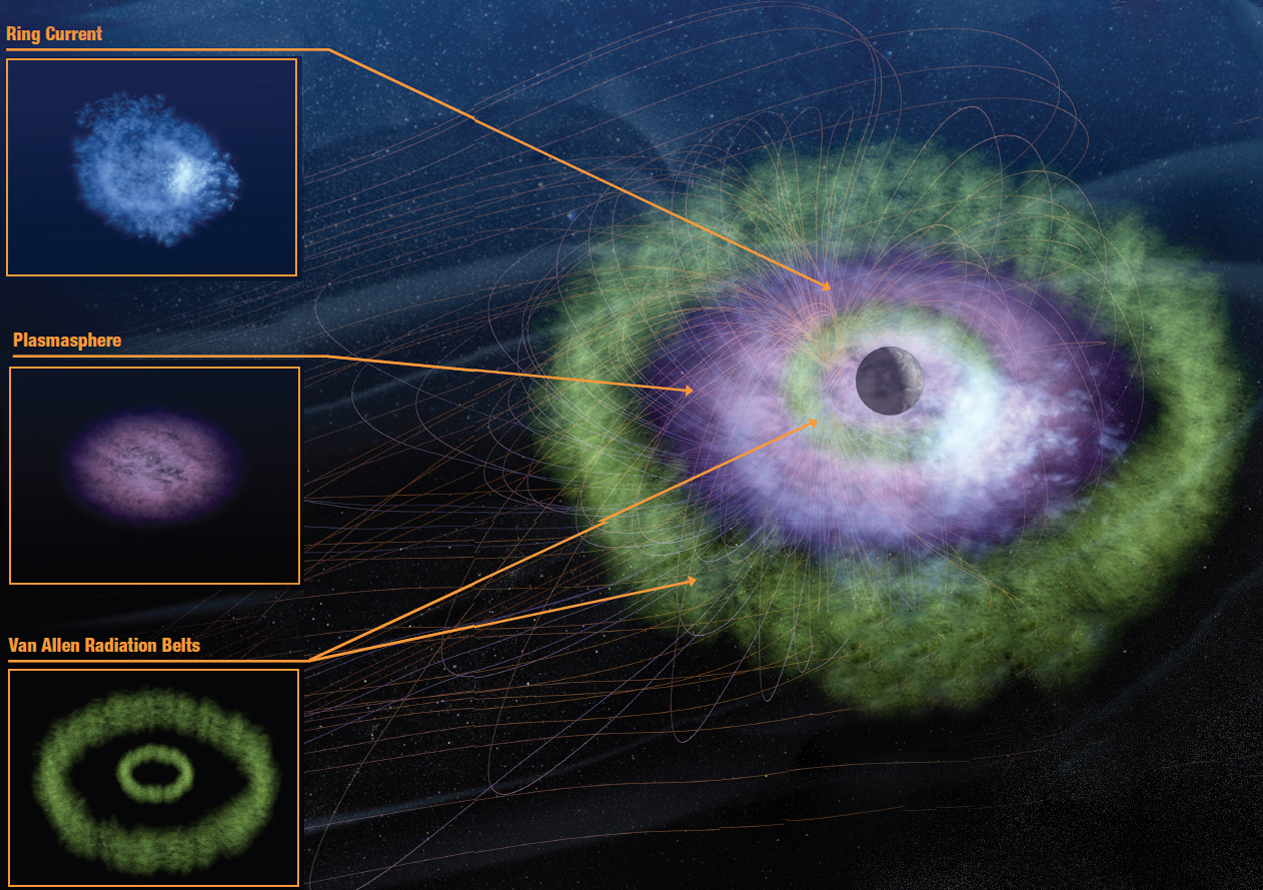
\includegraphics[scale=0.2]{{Figures/innermag-2.jpg}}
		\caption{Overview of inner magnetosphere. Adapted from NASA.}
		\label{fig:magnetosphereoverview}
	\end{figure}
\end{frame}


\begin{frame}
	\begin{figure}[htp]
		\centering
		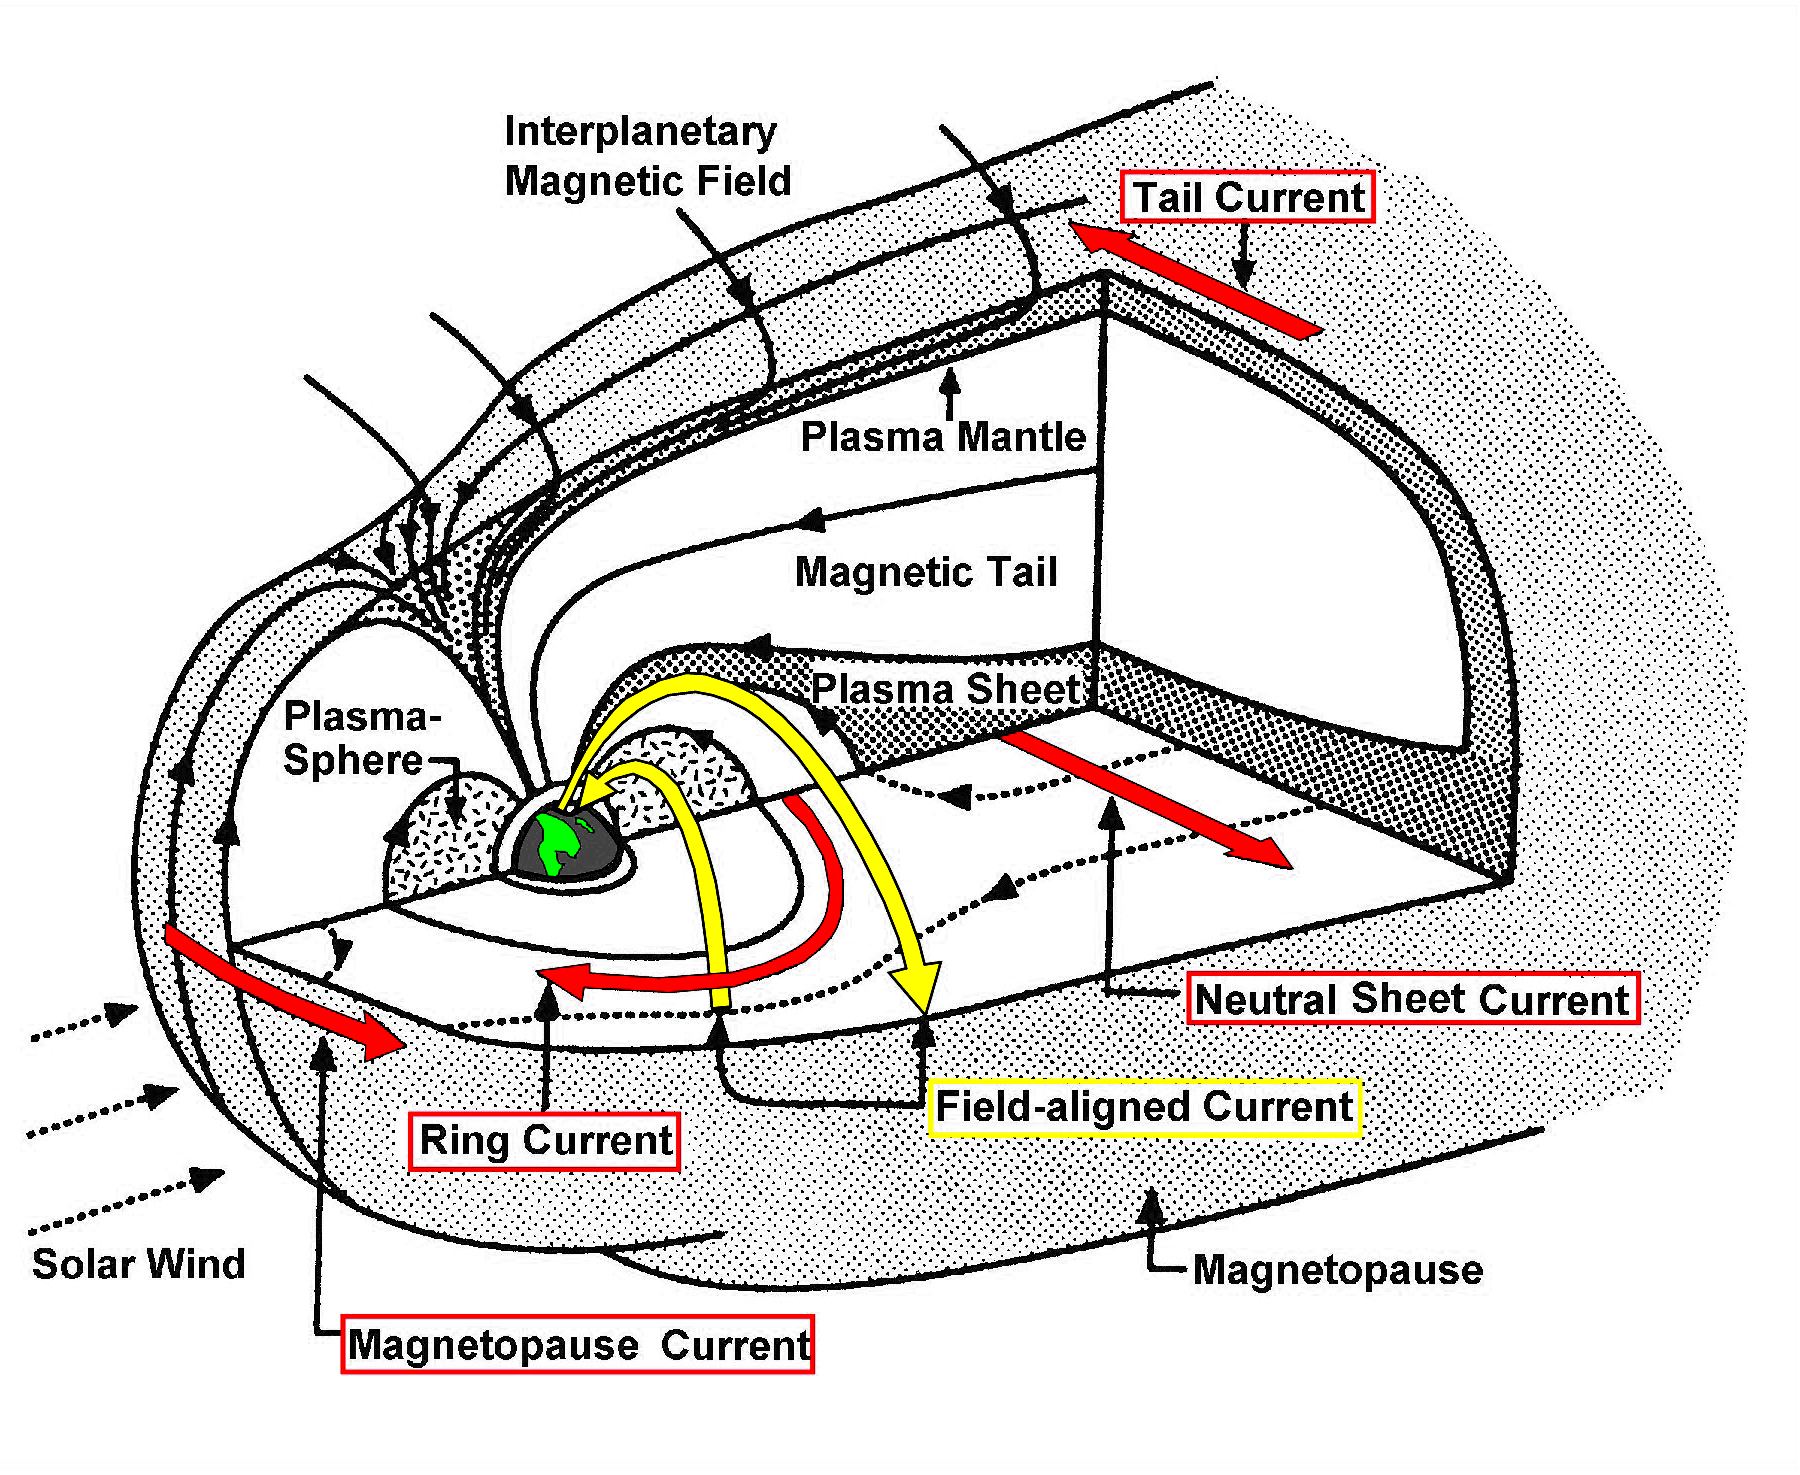
\includegraphics[scale=0.12]{{Figures/magnetosphere.jpg}}
		\caption{Currents in/around the magnetosphere. Adapted from Maus (2010).}
		\label{RingCurrentFigure}
	\end{figure}
\end{frame}



\subsection{Motivation}
\begin{frame}
	\begin{figure}
		\centering
		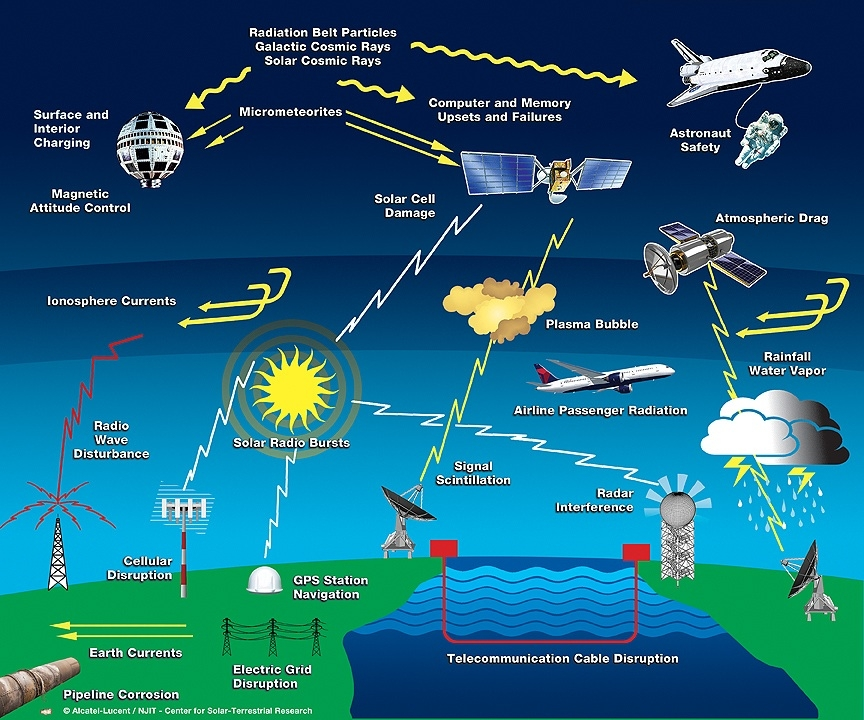
\includegraphics[width=0.75\linewidth]{Figures/TE_space_weather_diagram}
		\caption{Impacts of Space Weather [Lanzerotti]}
		\label{fig:TE_space_weather_diagram}
	\end{figure}
\end{frame}




\subsection{Data}

\begin{frame}
	\subheader
	Data used come from three sources:
	\small
	\begin{itemize}
		\item Denton (2007) for \req, MLT, and $AE$ \\
		\item King (2005) for \f
		\item Kondrashov (2014) for $B_z$, $V_{SW}$, Kp, $\rho_{sw}$, and $D_{st}$ \\
	\end{itemize}
\end{frame}

\begin{frame}
	Data coverage:
	\begin{itemize}
		\item Denton (2007): 10 minute, non-uniform, non-complete, from 1980-1991, GOES 2, 5, 6, and 7
		\item King (2005): 1 hour uniform, non-complete, from 1972-2013
		\item Kondrashov (2014): 1 hour uniform, complete, from 1972-2013
	\end{itemize}
\end{frame}


\begin{frame}
	How we measure geomagnetic activity:
	\begin{figure}[htp]
		\centering
		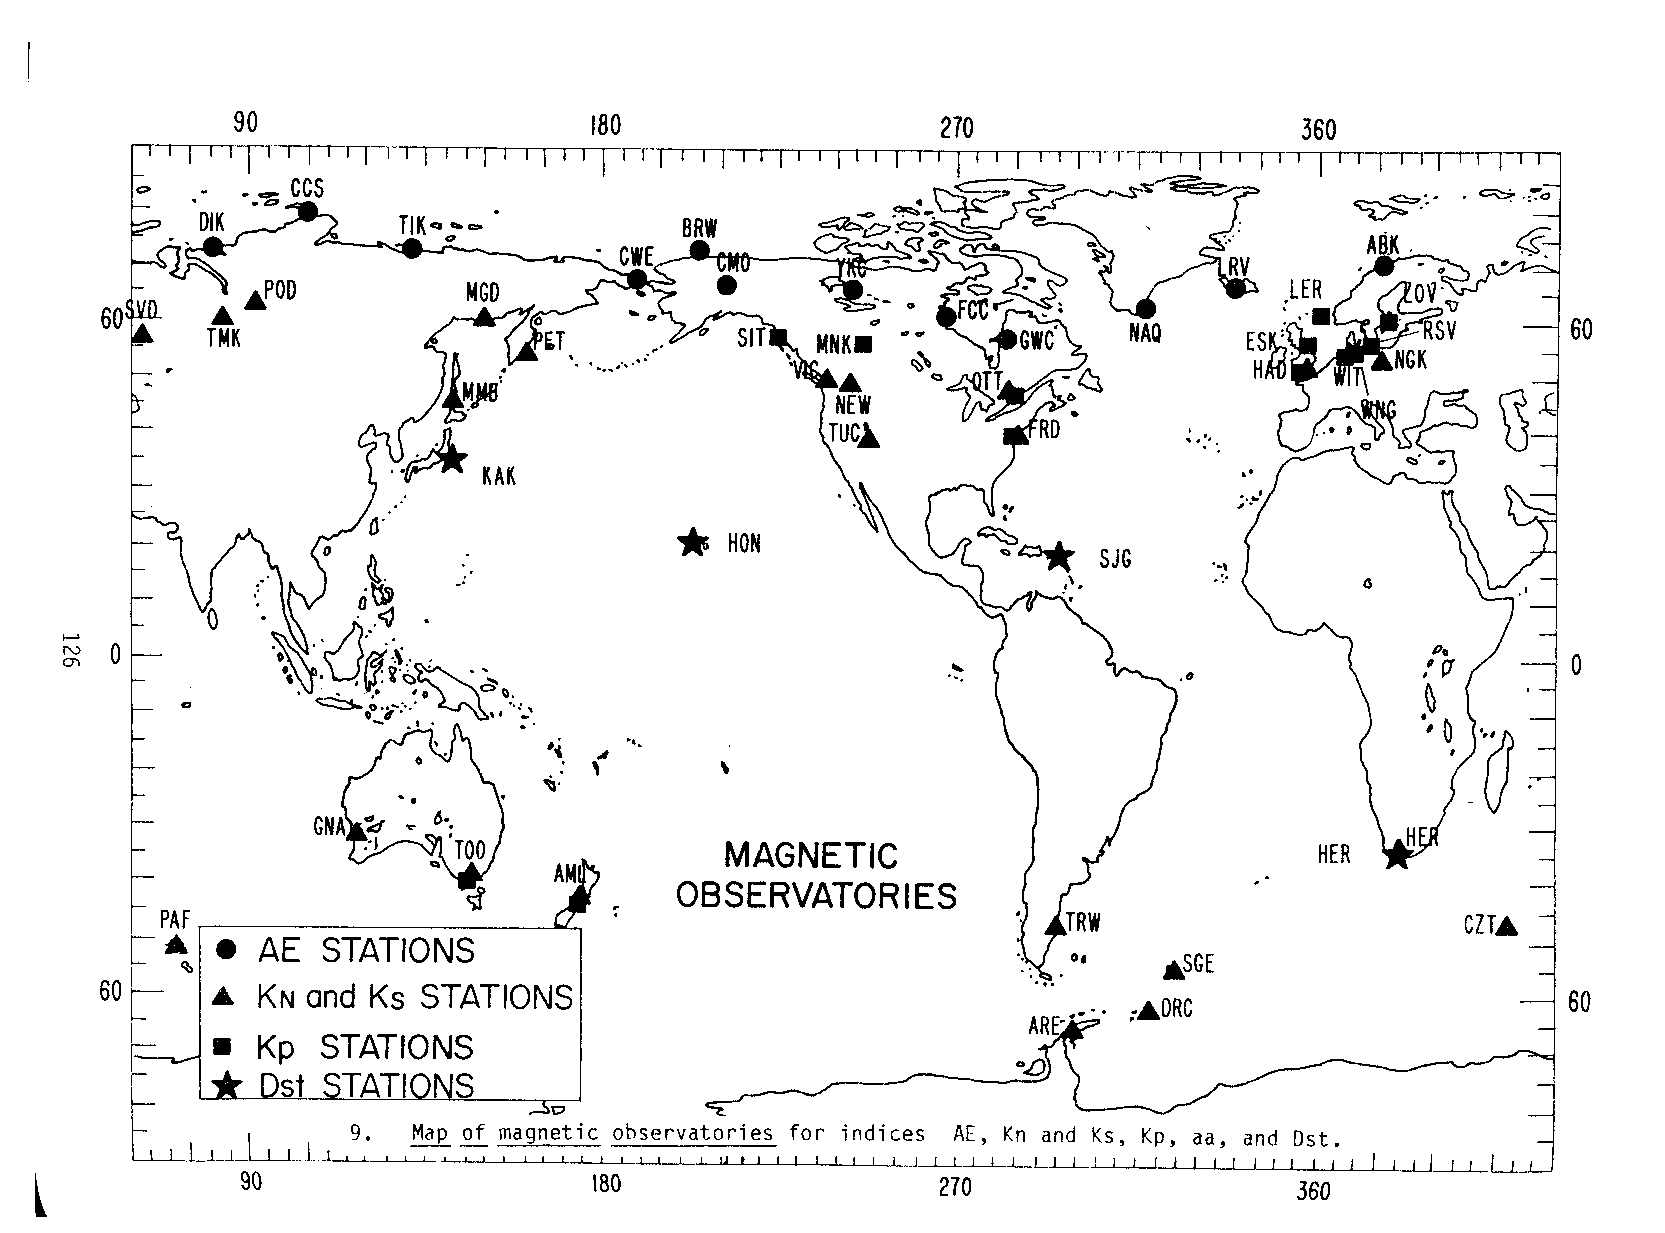
\includegraphics[scale=0.25]{{Figures/StationMap.eps}}
		\caption{Map of ground stations used to measure the $K_p$, $AE$, and \dst\ indices [Allen (1982)].}
		\label{fig:GroundStations}
	\end{figure}
\end{frame}

\begin{frame}
	\begin{figure}[htp!]
		\centering
		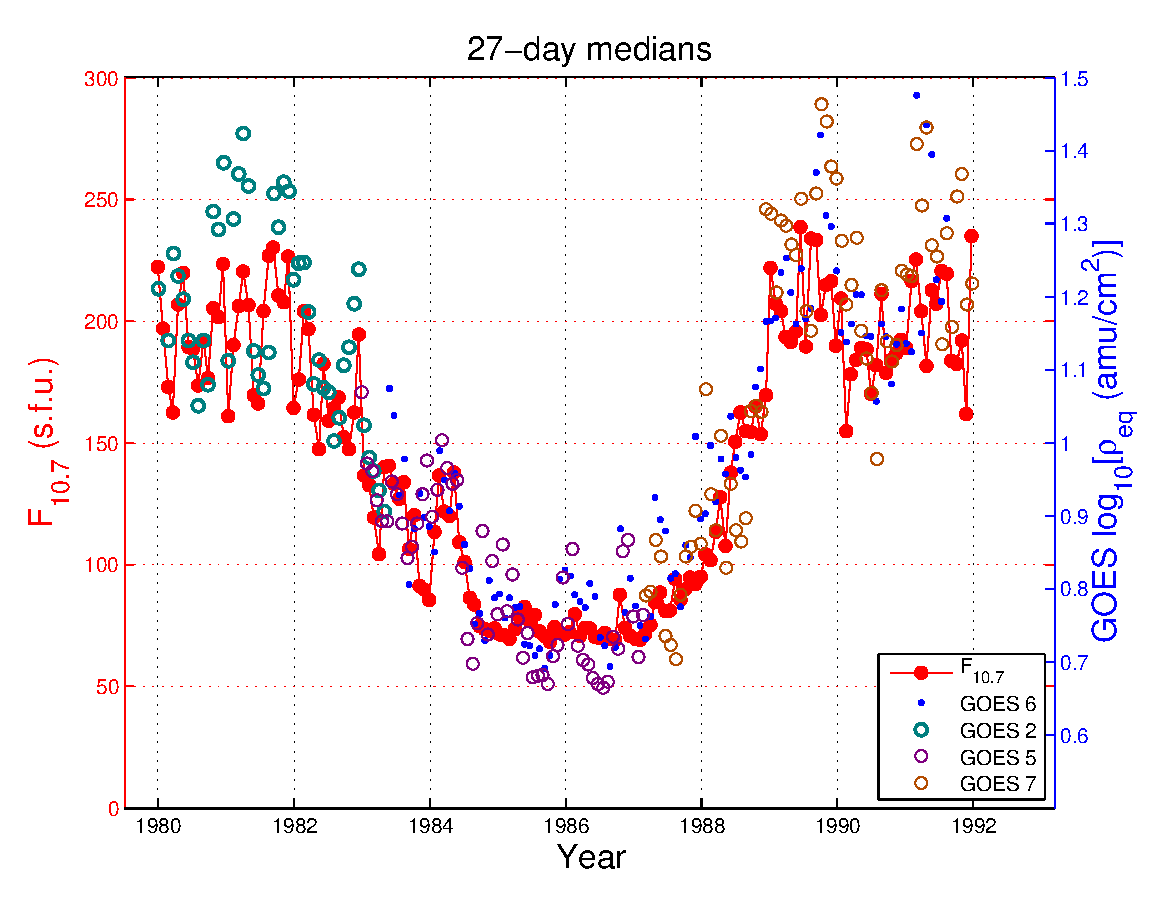
\includegraphics[width=0.95\linewidth]{Figures/F107MD27d-all}
		\caption{Comparing $F_{10.7\_27d}$ and $\log_{10}(\rho_{eq\_27d})$ using all available satellites.}
		\label{fig:F107rhoeq27dcomparison}
	\end{figure}
\end{frame}


\begin{frame}
	\begin{figure}[htp!]
		\centering
		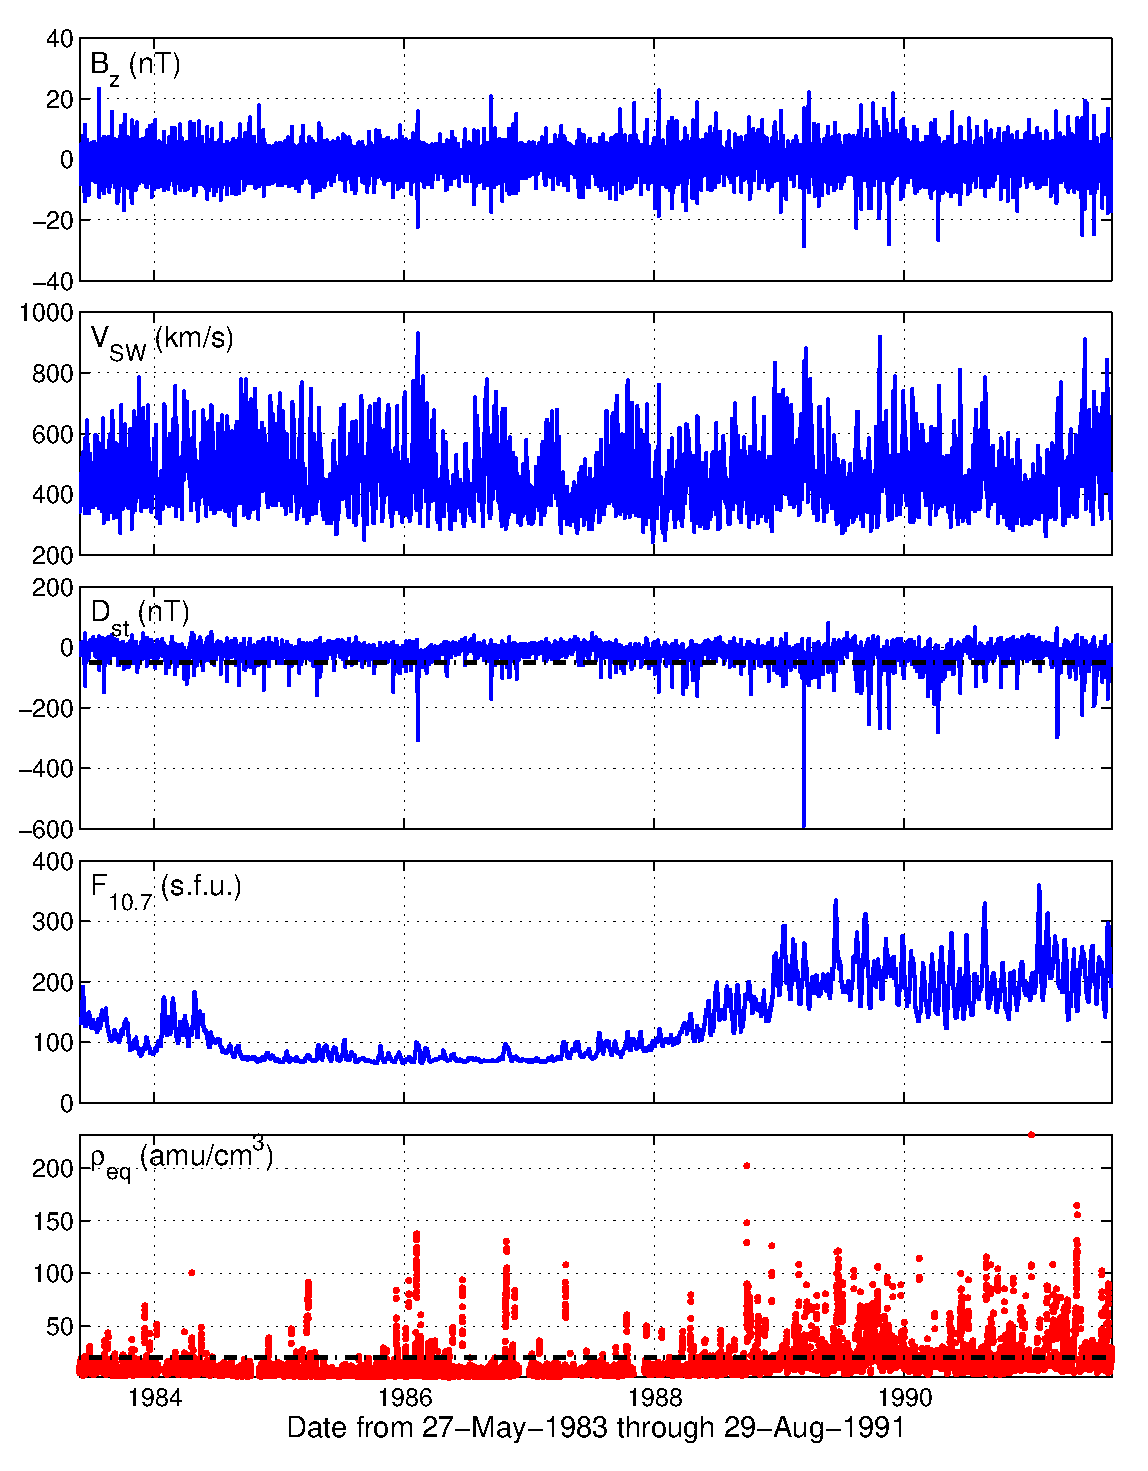
\includegraphics[width=0.5\linewidth]{Figures/alldata-GOES6-1983-1991}
		\caption{Data coverage with dashed lines indicating default event thresholds.}
		\label{fig:alldata-GOES6-1983-1991}
	\end{figure}
\end{frame}

\begin{frame}
	\req\ is derived from toroidal harmonic frequencies in the plasmatrough. Harmonics are not always detectable.
	\begin{figure}[htp!]
		\centering
		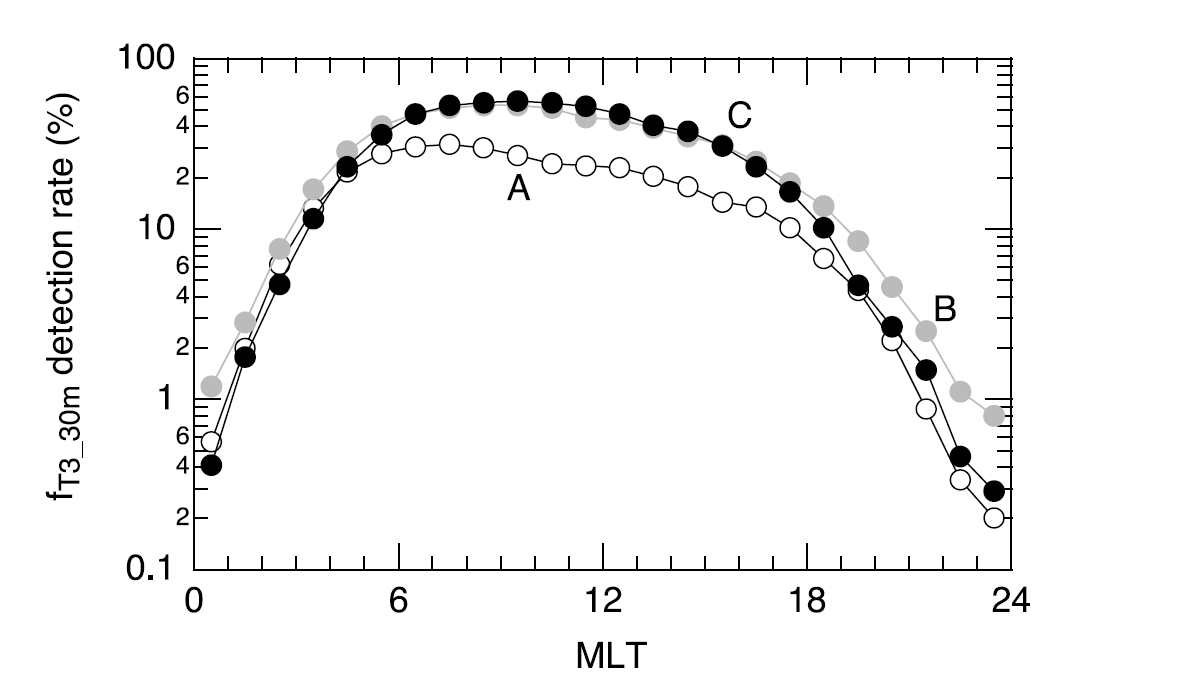
\includegraphics[width=0.4\linewidth]{Figures/Takahashi2010Availability.png}
		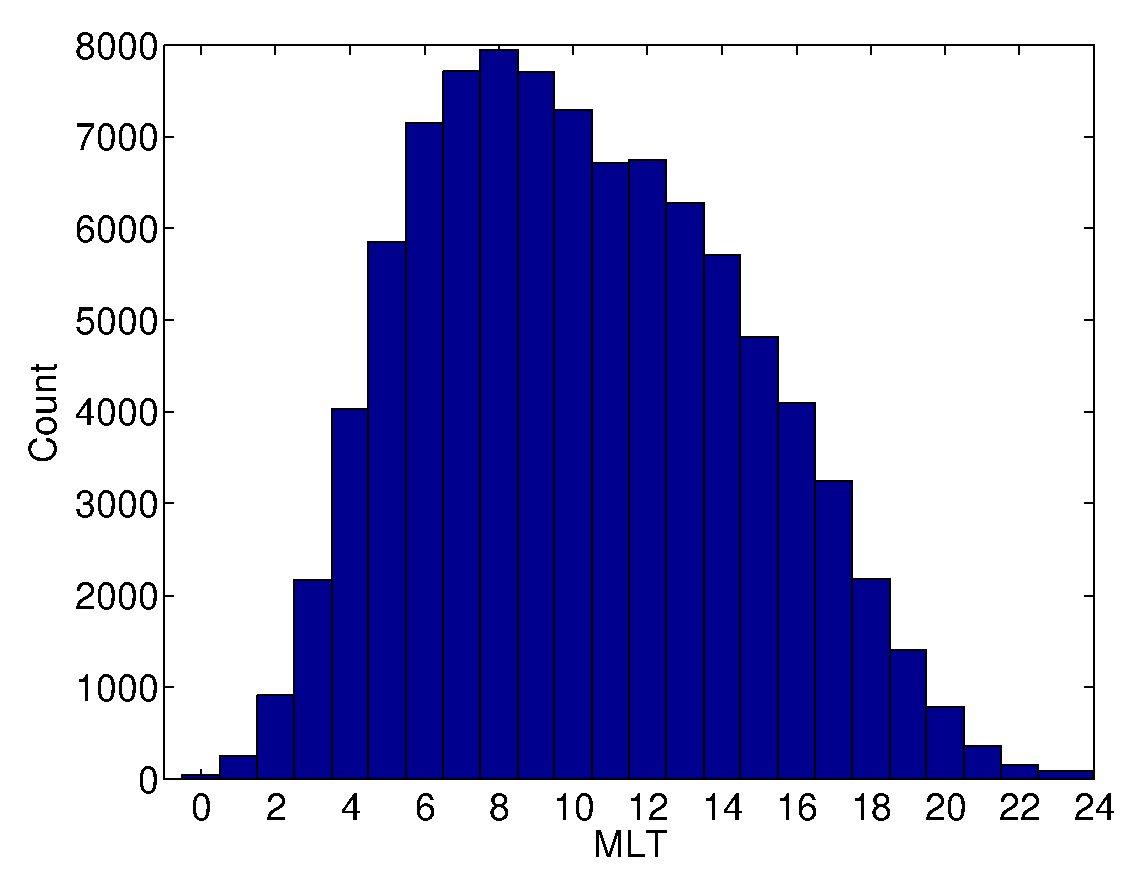
\includegraphics[width=0.4\linewidth]{Figures/databyMLT}
		\caption{Left: Detection rate of $f_{T3\_30m}$ for magnetic latitudes of 5, 9, and 11 degrees (curves A, B, and C respectively) [Takahashi (2010)]. Right: MLT of all available \req\ data.}
		\label{fig:Takahashi2010Availability}
	\end{figure}
\end{frame}

\begin{frame}
\begin{figure}[htp!]
	\centering
	\includegraphics[width=0.5\linewidth]{Figures/alldata-GOES6-10Mar1989-17Mar1989.eps}%alldata-GOES6-1989-1989}
	\caption{Data from GOES 6 around March 1989 geomagnetic storm.}
	\label{fig:alldata-GOES6-1989-1989}
\end{figure}
\end{frame}



\begin{frame}
	\begin{figure}[htp!]
		\centering
		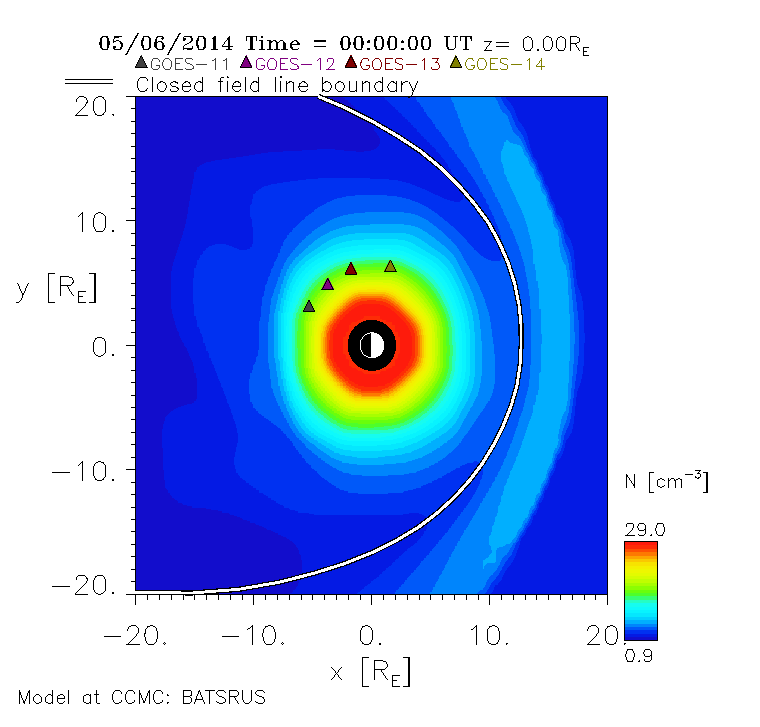
\includegraphics[width=0.45\linewidth]{Figures/idl_798387073825_050215_2_20140506_000000_before}
		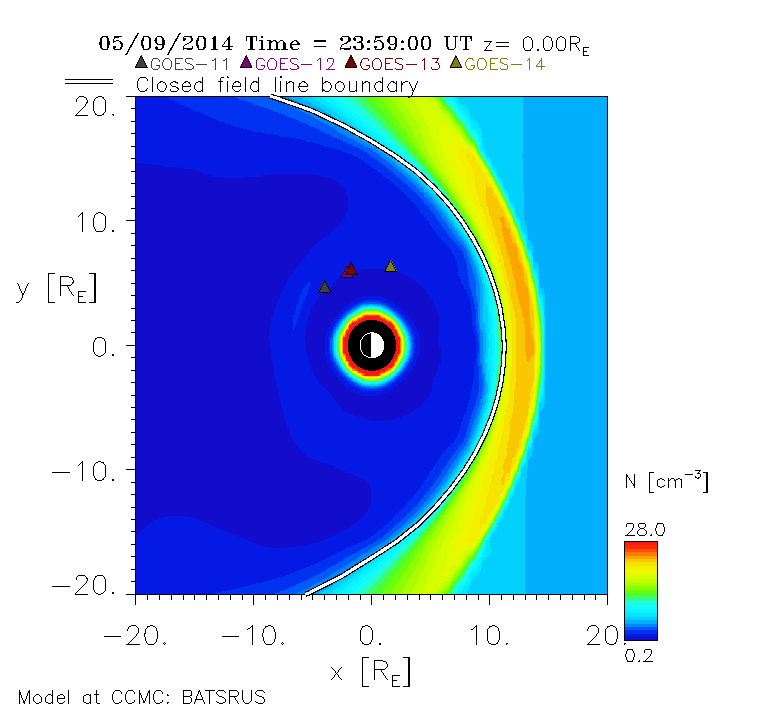
\includegraphics[width=0.45\linewidth]{Figures/idl_798605093993_050215_2_20140509_235900_after}
		\caption{Model of magnetopause/plasmasphere before and after geomagnetic activity, showing location of GOES satellites in geosynchronous orbit [CCMC].}
		\label{fig:PlasmapauseLocation}
	\end{figure}
\end{frame}

%http://iswa.ccmc.gsfc.nasa.gov/IswaSystemWebApp/index.jsp?i_1=1&l_1=18&t_1=152&w_1=500&h_1=400&s_1=2014-05-09%2021:34:36.0_0_10_3&i_2=41&l_2=47&t_2=607&w_2=542&h_2=481&s_2=2014-05-09%2021:57:48.0_0_10_3&i_3=44&l_3=591&t_3=780&w_3=500&h_3=333&s_3=2014-05-09%2021:49:48.0_0_10_3&i_4=335&l_4=1094&t_4=725&w_4=800&h_4=400&s_4=2014-05-09%2019:30:00.0!3!&i_5=39&l_5=1370&t_5=325&w_5=500&h_5=333&s_5=2014-05-09%2021:49:48.0_0_10_3&i_6=443&l_6=597&t_6=121&w_6=720&h_6=586&s_6=2014-05-09%2021:58:00.0_0_10_3

%http://ccmc.gsfc.nasa.gov/results/viewrun.php?domain=GM&runnumber=Lois_Smith_050215_2

\begin{frame}
	\begin{figure}[htp!]
		\centering
		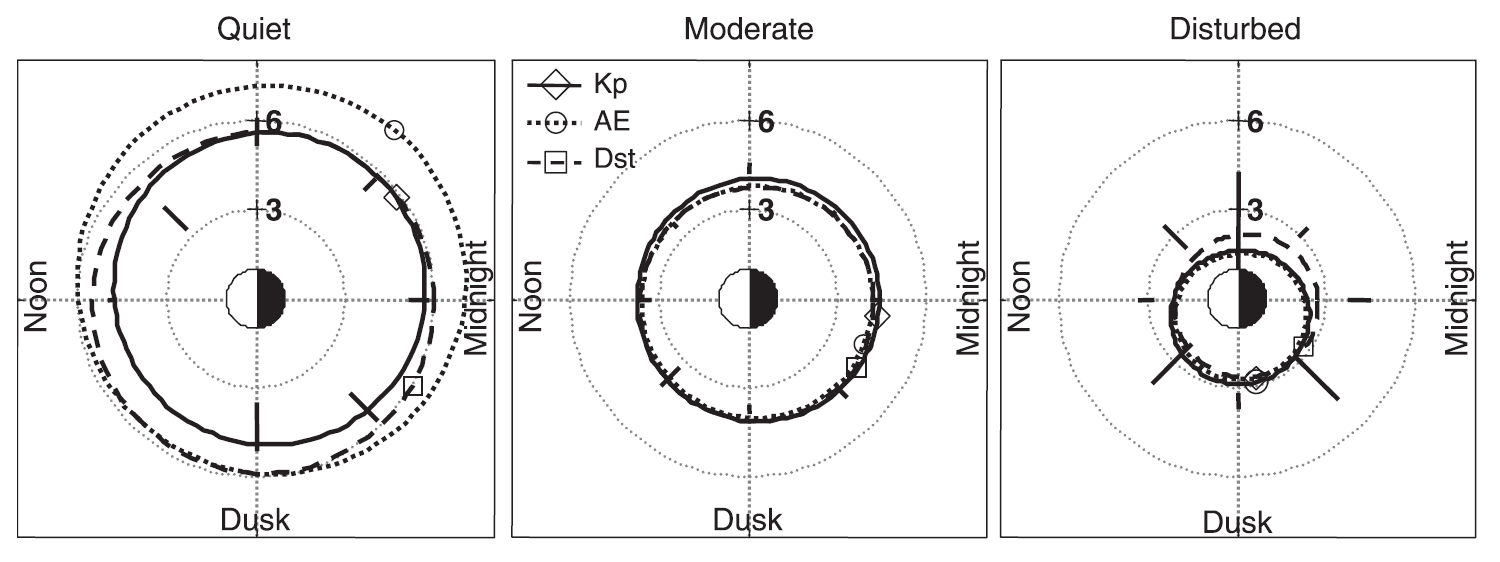
\includegraphics[width=0.9\linewidth]{Figures/PlasmapauseLocation.png}
		\caption{Model of plasmapause location as it varies with geomagnetic activity where the symbols indicate the local time of maximum plasmapause location [O'Brien and Moldwin (2003)].}
		\label{fig:PlasmapauseLocation}
	\end{figure}
\end{frame}

\begin{frame}
	\begin{figure}[htp]
		\centering
		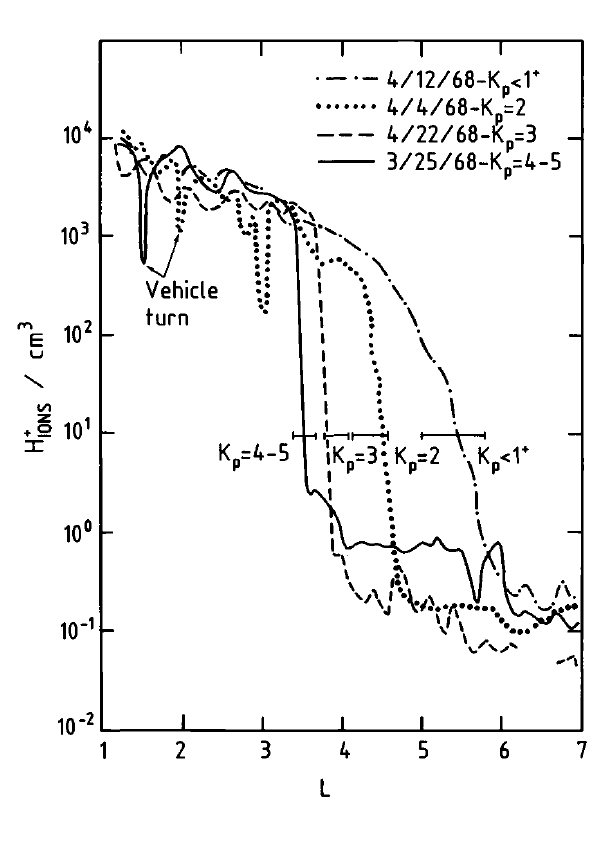
\includegraphics[scale=0.2]{{Figures/LemairePlasmapauseKnee.png}}
		\caption{Plasmapause position varying with $K_p$ as represented by several particular plasmapause crossings made on outbound passes between local times of midnight and 0400 [Lemaire (1998)].}
		\label{fig:LemaireKnee}
	\end{figure}
\end{frame}


\subsection{Questions}
\begin{frame}
	\subheader
	Questions addressed by this dissertation:
	\begin{itemize}
		\item What enhances \req\ in the plasmatrough? Solar wind (via geomagnetic storms) or internal processes (e.g. ionospheric outflow)?
		\item Does a \req\ enhancement depend on current IMF conditions?
		\item Can a \req\ enhancement be classified or forecasted?
	\end{itemize}
\end{frame}






%%%%%%%%%%%%%%%%%%%%%%%%%%%%%%%%%%%%%%%%%%%%%%%%%%%
%___  ___     _   _               _       _                   
%|  \/  |    | | | |             | |     | |                  
%| .  . | ___| |_| |__   ___   __| | ___ | | ___   __ _ _   _ 
%| |\/| |/ _ \ __| '_ \ / _ \ / _` |/ _ \| |/ _ \ / _` | | | |
%| |  | |  __/ |_| | | | (_) | (_| | (_) | | (_) | (_| | |_| |
%\_|  |_/\___|\__|_| |_|\___/ \__,_|\___/|_|\___/ \__, |\__, |
%											       __/ | __/ |
%										          |___/ |___/ 
%%%%%%%%%%%%%%%%%%%%%%%%%%%%%%%%%%%%%%%%%%%%%%%%%%%

\section{Methodology}
\begin{frame}
Four main methods of analysis used:
\begin{enumerate}
	\item Linear/Auto-Regressive with exogenous inputs (ARX) 
	\item Nonlinear Neural Network
	\item Epoch
	\item Nonlinear Classification and Prediction
\end{enumerate}
\end{frame}

\subsection{Linear and ARX}

\begin{frame}
	\subheader
	Linear uses Ordinary Least Squares on model of form $y=AX+c+\varepsilon$ with median of four hours before onset as X. 
\newline

	ARX starts with Box-Jenkins model:
	\begin{align*}
	x(t)&=\sum_{j=1}^{m}{b_j \cdot f(t-j\Delta t)}+c + \varepsilon_t
	\end{align*}
	Modified to be an autoregressive model with exogenous inputs (ARX):
	\begin{align*}
	\hat{x}(t)&=\sum_{i=1}^la_i\cdot x(t-i\Delta t)+\sum_{j=1}^m b_j\cdot f(t-j\Delta t)+c+\varepsilon_t
	\label{ARXEqn}
	\end{align*}
\end{frame}


\begin{frame}
	Resultant matrix to solve:
        \[
        \left( \begin{array}{ccccccc}
        x_0 & ... & x_{\tau-1} & f_0 & ... & f_{\tau-1} & 1\\
        x_1 &     & x_\tau & f_\tau &  &f_\tau & 1\\
        ... &     &     &     &  &   & \\
        x_{N-\tau} & ... & x_{N-1} & f_{N-\tau} & ... & f_{N-1} & 1
        \end{array} \right)
        \left(\begin{array}{c}
        a_0\\...\\a_{\tau-1}\\b_0\\...\\b_{\tau-1}\\c
        \end{array}\right)
        =
        \left(                                                                                                                                                                                    
        \begin{array}{c}
        x_\tau \\ x_{\tau+1} \\ ... \\ x_{N}
        \end{array}
        \right)
        \]
\end{frame}

\begin{frame}
	\begin{figure}[htp]
		\centering
		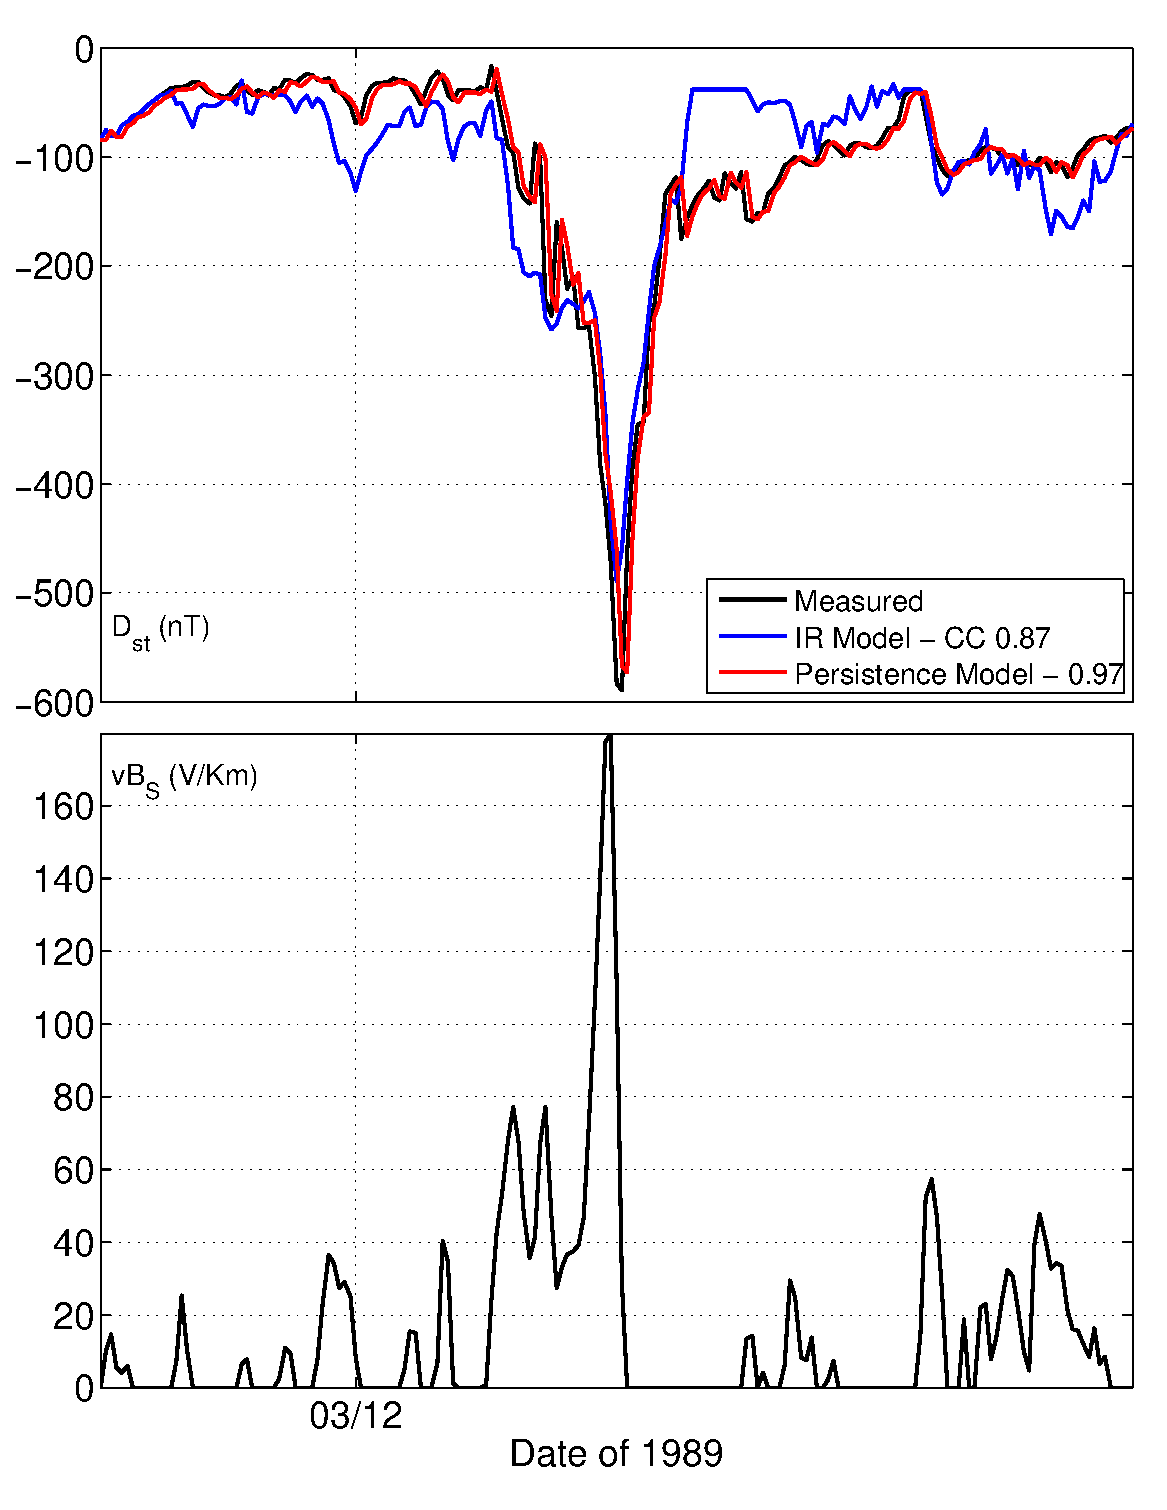
\includegraphics[scale=0.25]{{Figures/BasicModelExample-GOES6}}
		\caption{Top: \dst\ (black), persistence (red), 12-hour impulse response model (blue). Bottom: $vB_S$ input.}
		\label{VBzIRplot}
	\end{figure}
\end{frame}


\subsection{Neural Network}

\begin{frame}
	\subheader
	Neural Network model benefits:
	\begin{enumerate}
		\item Can model nonlinear effects
		\item Easily adaptable to binary classification
	\end{enumerate}
	Neural Network model disadvantages:
	\begin{enumerate}
		\item Susceptible to overfitting
		\item More complex to create and analyze
		\item No closed-form optimum solution
	\end{enumerate}
\end{frame}


\begin{frame}
	Example nonlinear effect:
	\begin{figure}[htp!]
		\centering
		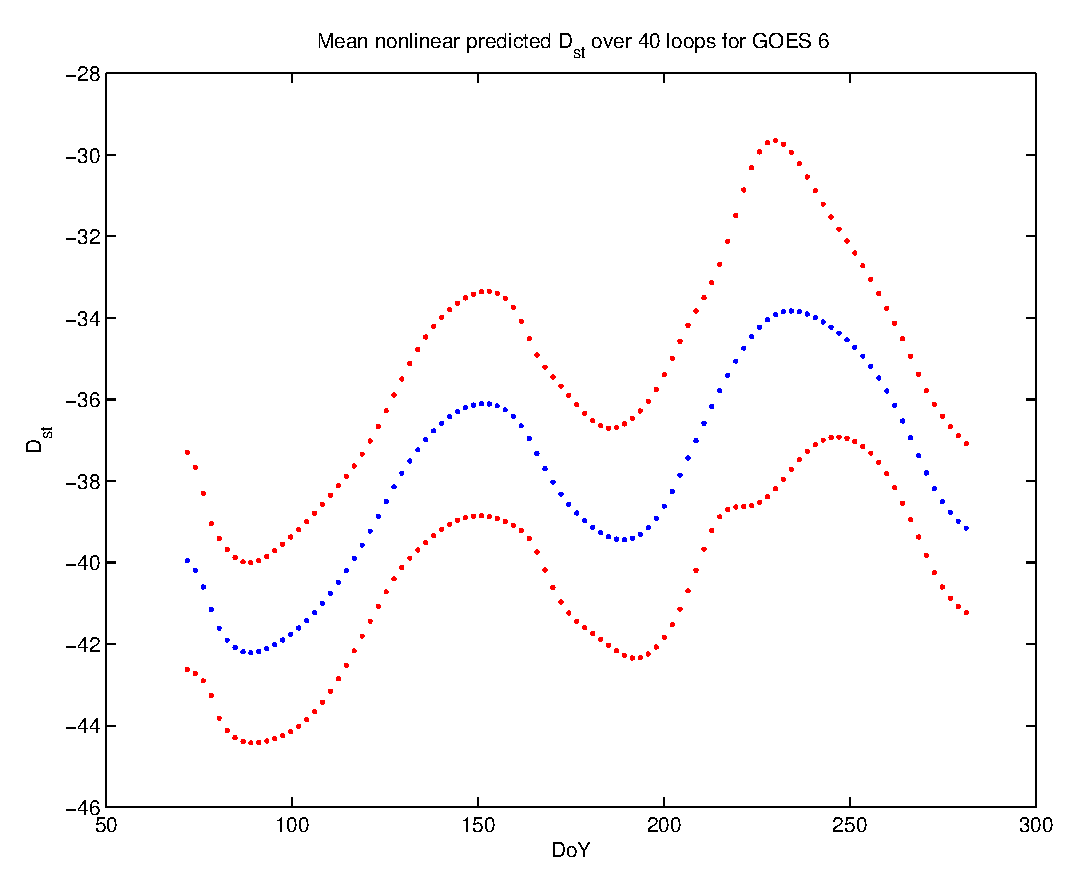
\includegraphics[width=0.7\linewidth]{Figures/NNDoY-Dst-GOES6}	
		\caption{\dst\ predicted by nonlinear model of day of year.}
		\label{fig:DoYDst}
	\end{figure}
\end{frame}




\subsection{Epoch}
\begin{frame}
	\subheader
	Epoch Analyses average multiple events to find underlying patterns.
\begin{figure}
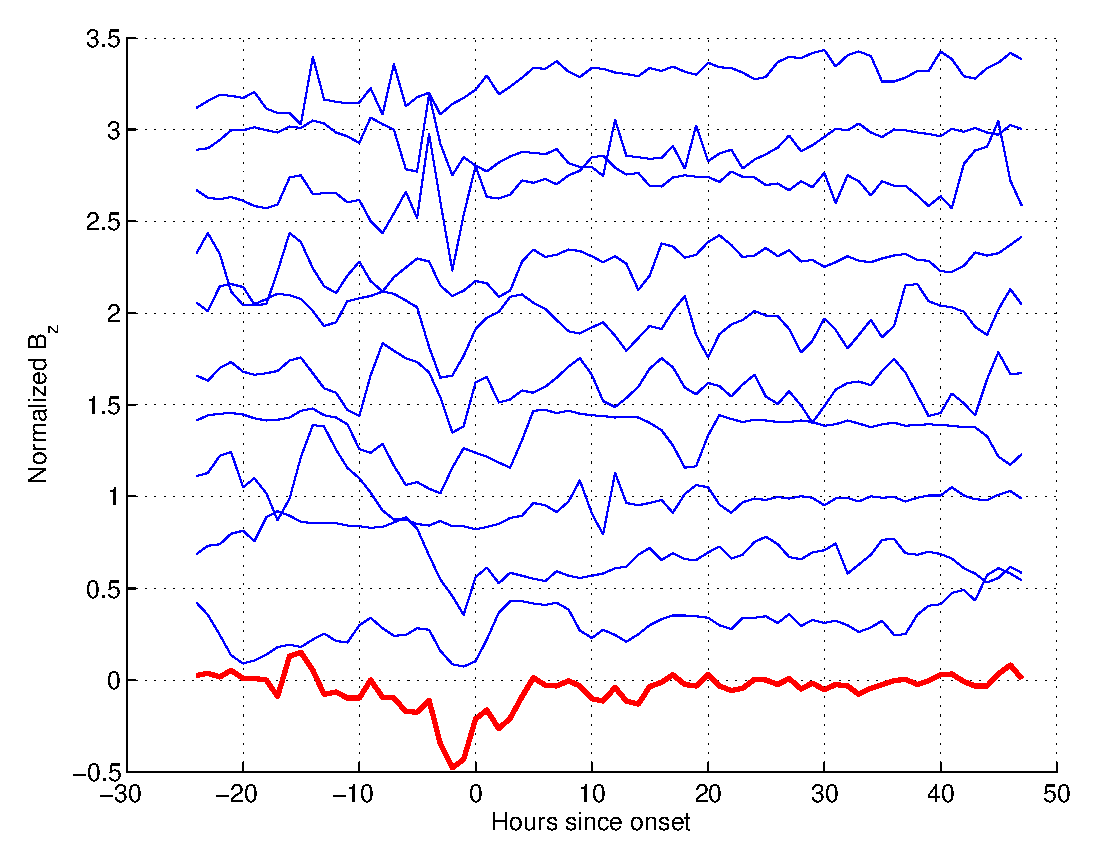
\includegraphics[scale=0.3]{Figures/epochexample}
\caption{Sample epoch analysis showing ten events (blue) and their median (red)}
\label{fig:epochexample}
\end{figure}
\end{frame}



\subsection{Classification and Prediction}

\begin{frame}
	\subheader
	Is an onset distinguishable using just the variables provided?
	\begin{figure}[htp!]
		\centering
		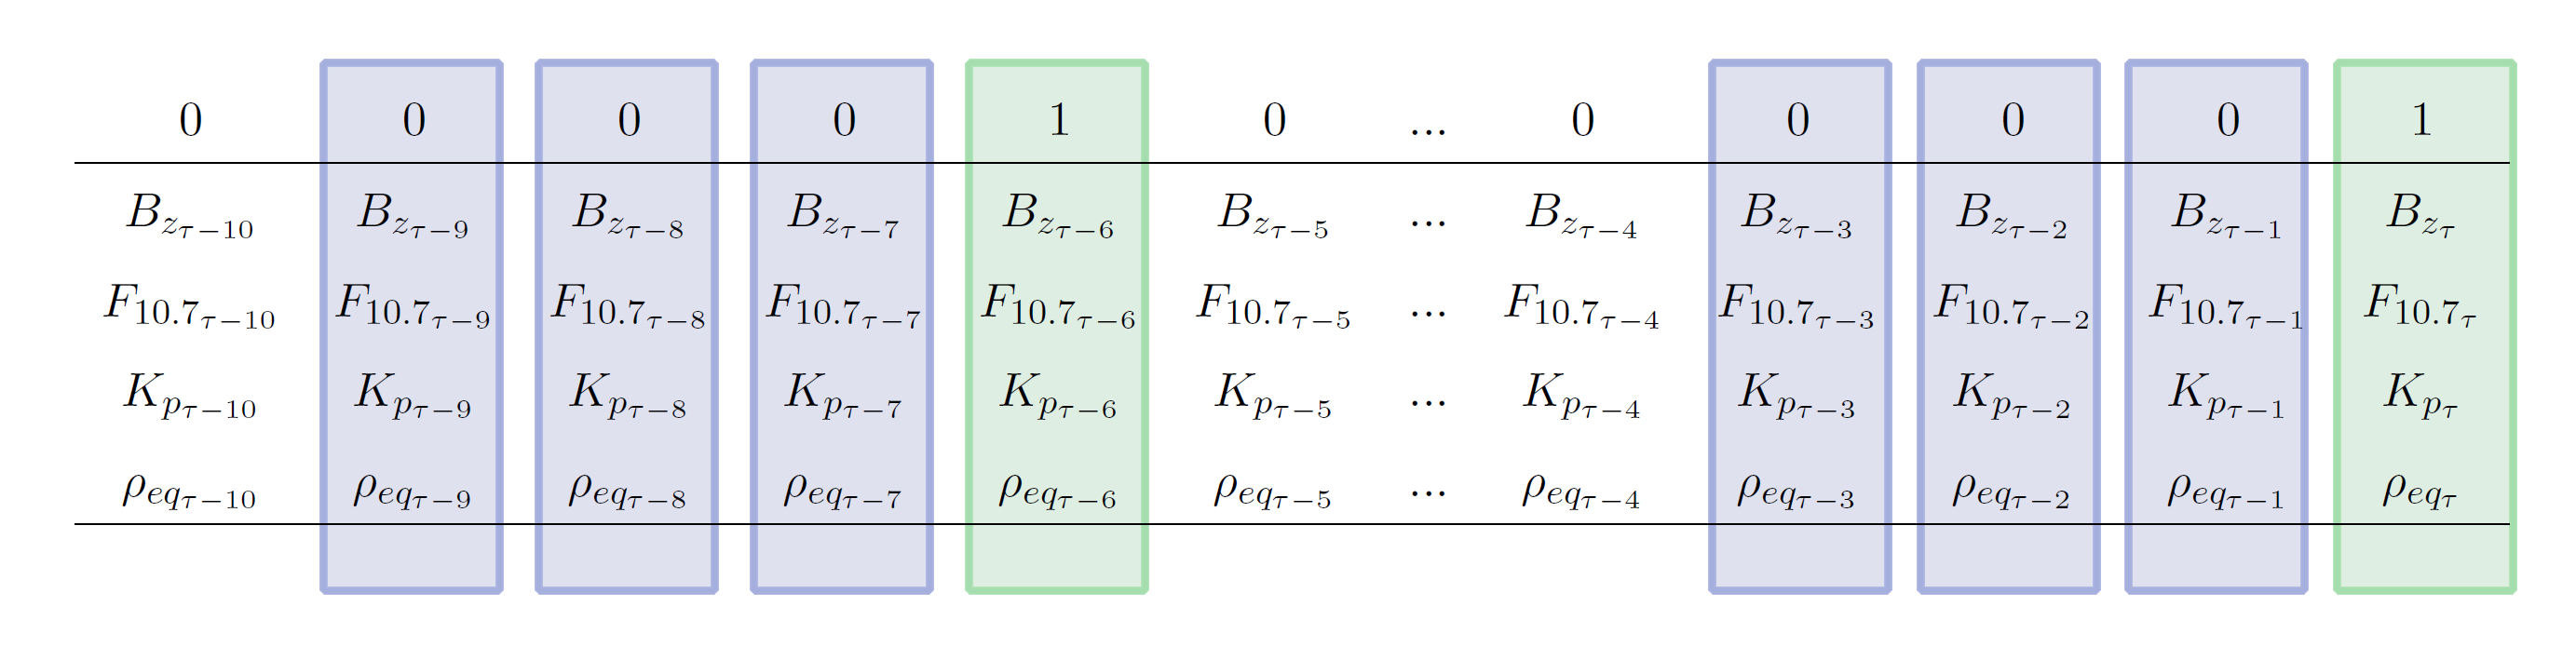
\includegraphics[width=1\linewidth]{Figures/CH5/ClassifyGraphic-2.png}
		\caption{Diagram of classification method.}
		\label{fig:ClassifyDiagram}
	\end{figure}
\end{frame}


\begin{frame}
	Can an onset be forecasted using the previous four hours or days?
	\begin{figure}[htp!]
		\centering
		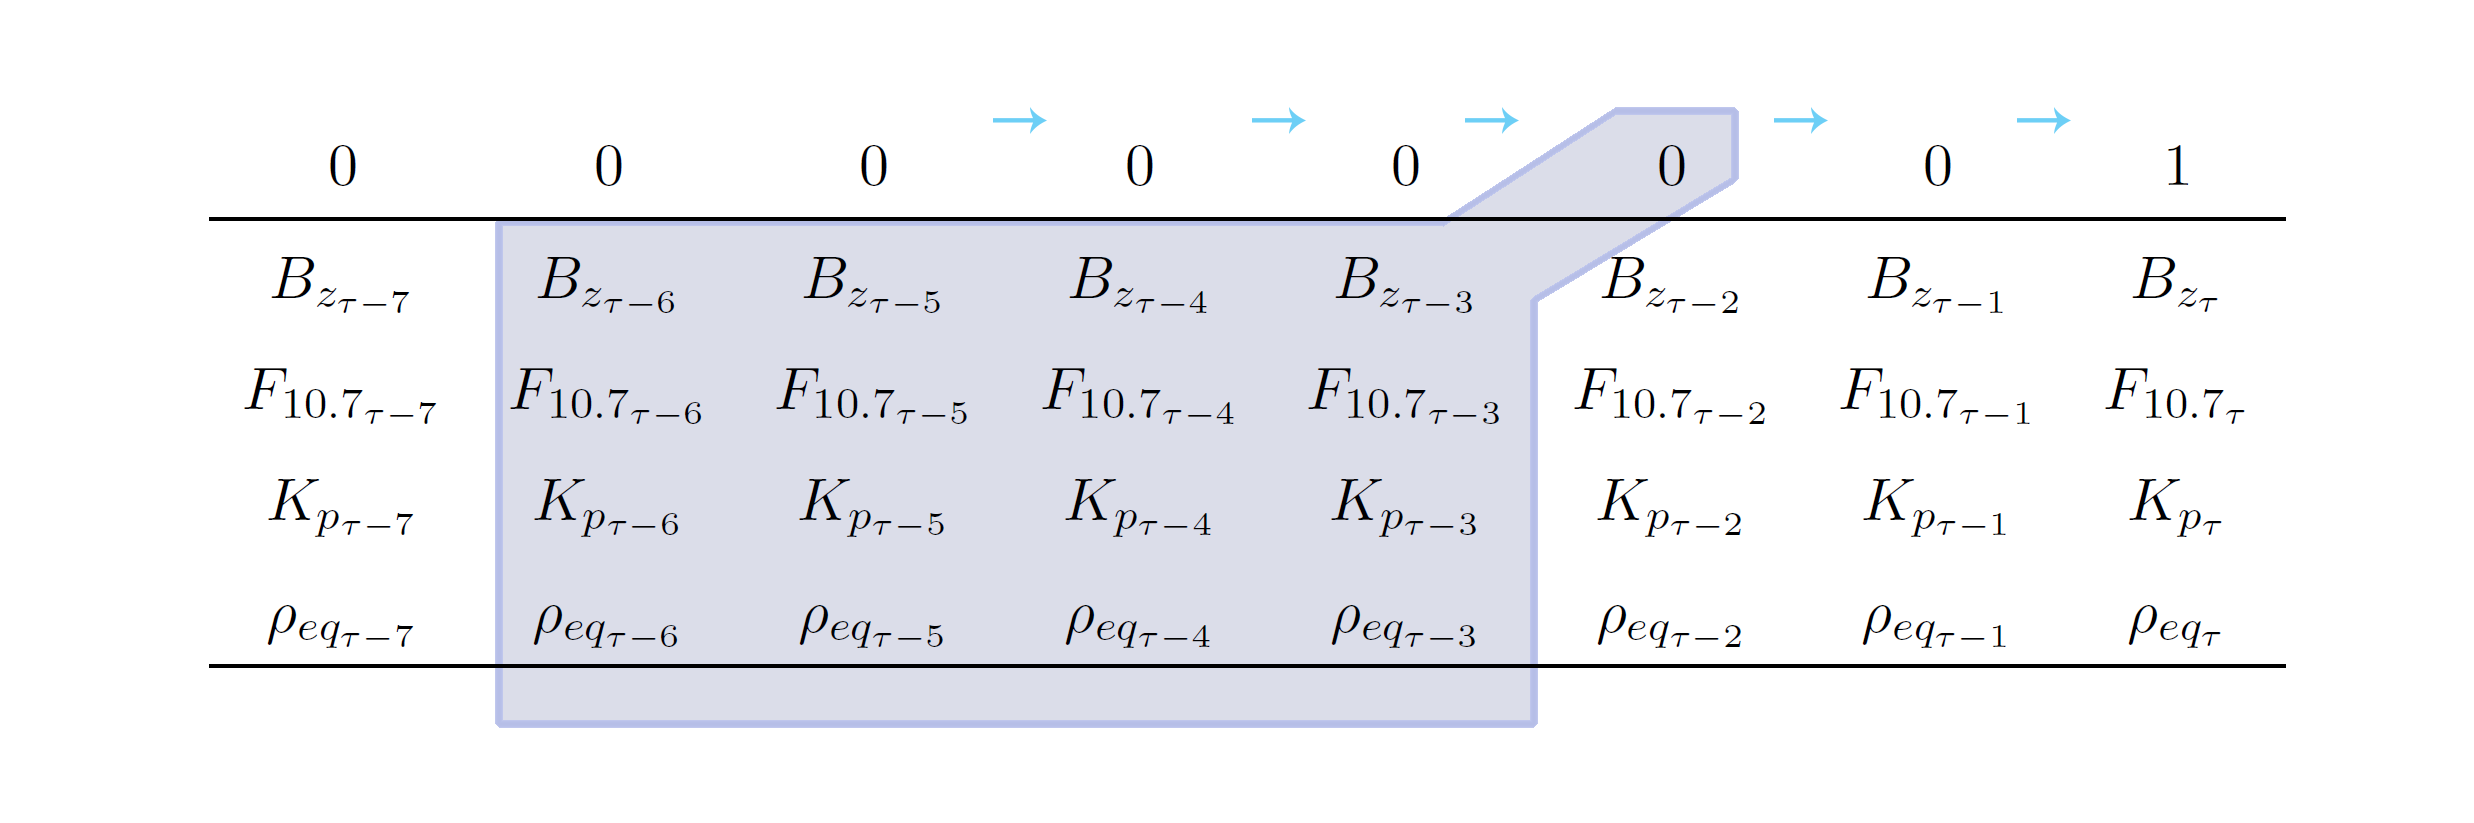
\includegraphics[width=1\linewidth]{Figures/CH5/FullGraphic-2.png}
		\caption{Diagram of prediction method.}
		\label{fig:ClassifyDiagram}
	\end{figure}
	
	
\end{frame}

%%%%%%%%%%%%%%%%%%%%%%%%%%%%%%%%%%%%%%%%%%%%%%%%%%%
%______               _ _       
%| ___ \             | | |      
%| |_/ /___ ___ _   _| | |_ ___ 
%|    // _ / __| | | | | __/ __|
%| |\ |  __\__ | |_| | | |_\__ \
%\_| \_\___|___/\__,_|_|\__|___/
%%%%%%%%%%%%%%%%%%%%%%%%%%%%%%%%%%%%%%%%%%%%%%%%%%%
\section{Results}
\subsection{Traditional Models}

\begin{frame}
	\subheader
	\begin{table}[h]
		\footnotesize
		\begin{tabular}{|C|CCC|}
			\hline
                         &  Linear & Nonlinear  & ARX_{24} \\ \hline
                         DoY  &  -0.06\pm0.06  & +0.32\pm0.22 & +0.04 \\
                         MLT  &  +0.01\pm0.23  & +0.40\pm0.32 & +0.27 \\
                         \rowcolor{lightgray} B_z  &  +0.08\pm0.14  & +0.17\pm0.19 & +0.22 \\
                         V_{sw}  &  +0.06\pm0.11  & +0.19\pm0.24 & +0.21 \\
                         D_{st}  &  +0.06\pm0.13  & +0.02\pm0.17 & +0.05 \\
                         \rho_{sw}  &  +0.12\pm0.19  & +0.20\pm0.22 & +0.08 \\
                         \rowcolor{lightgray}F_{10.7}  &  +0.51\pm0.06  & +0.48\pm0.25 & +0.45 \\
                         B_z+V_{sw}  &  +0.12\pm0.10  & +0.15\pm0.21 & +0.29 \\
                         \rowcolor{lightgray}B_z+\f & +0.56\pm0.16 & +0.46\pm0.21 &  +0.49 \\
                         D_{st}+F_{10.7}  &  +0.54\pm0.07  & +0.47\pm0.15 & +0.46 \\
                         \rowcolor{lightgray}All  &  +0.61\pm0.11  & +0.60\pm0.35 & +0.61 \\
			\hline
		\end{tabular}
		\caption{Table of linear model test-set correlations showing the median of 100 random samples. Each sample trained on half of the data (via randomly selected rows of the least squares matrix) and tested on the other half.} 
		\label{CCperltable}
	\end{table}
\end{frame}

\begin{frame}
	\begin{itemize}
		\item Nonlinear has more variation in samples, and between test and training sets, but does well for nonlinear variables such as DoY and MLT
		\item Can see that \f\ is the dominant source of correlation for all models
		\item Other variables are highly collinear 
		\item Even using a model of all variables barely accounts for half of \req.
		\item Previous studies make more complex models or focus on fewer events; this dissertation attempts epoch analysis
	\end{itemize}

\end{frame}



\subsection{Epoch}

\begin{frame}
	\subheader
	Epoch Analysis performed on two types of events:
	\begin{itemize}
		\item $\req >$ 20 amu/cm$^3$
		\item $\dst <$ -50 nT
	\end{itemize}
	Threshold crossings for events considered at an hourly timescale.
	\newline
	
	Linear interpolation done on \req\ to approximate event onsets when lacking data, but left as fill-values for analysis. 
\end{frame}


\begin{frame}
	\begin{figure}[htp!]
		\centering
		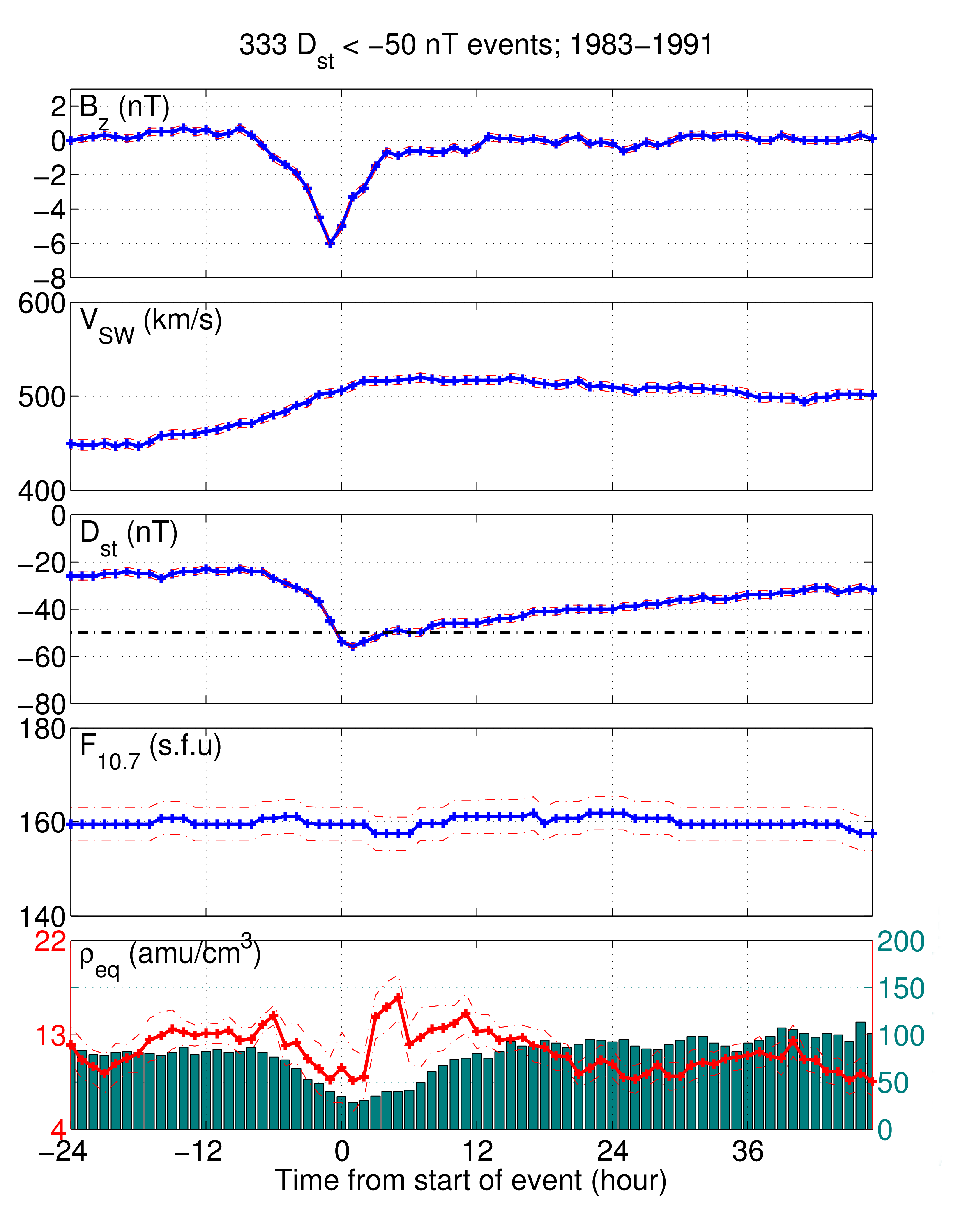
\includegraphics[width=0.5\linewidth]{Figures/StormAvs/stormavs-dst-GOES6}
		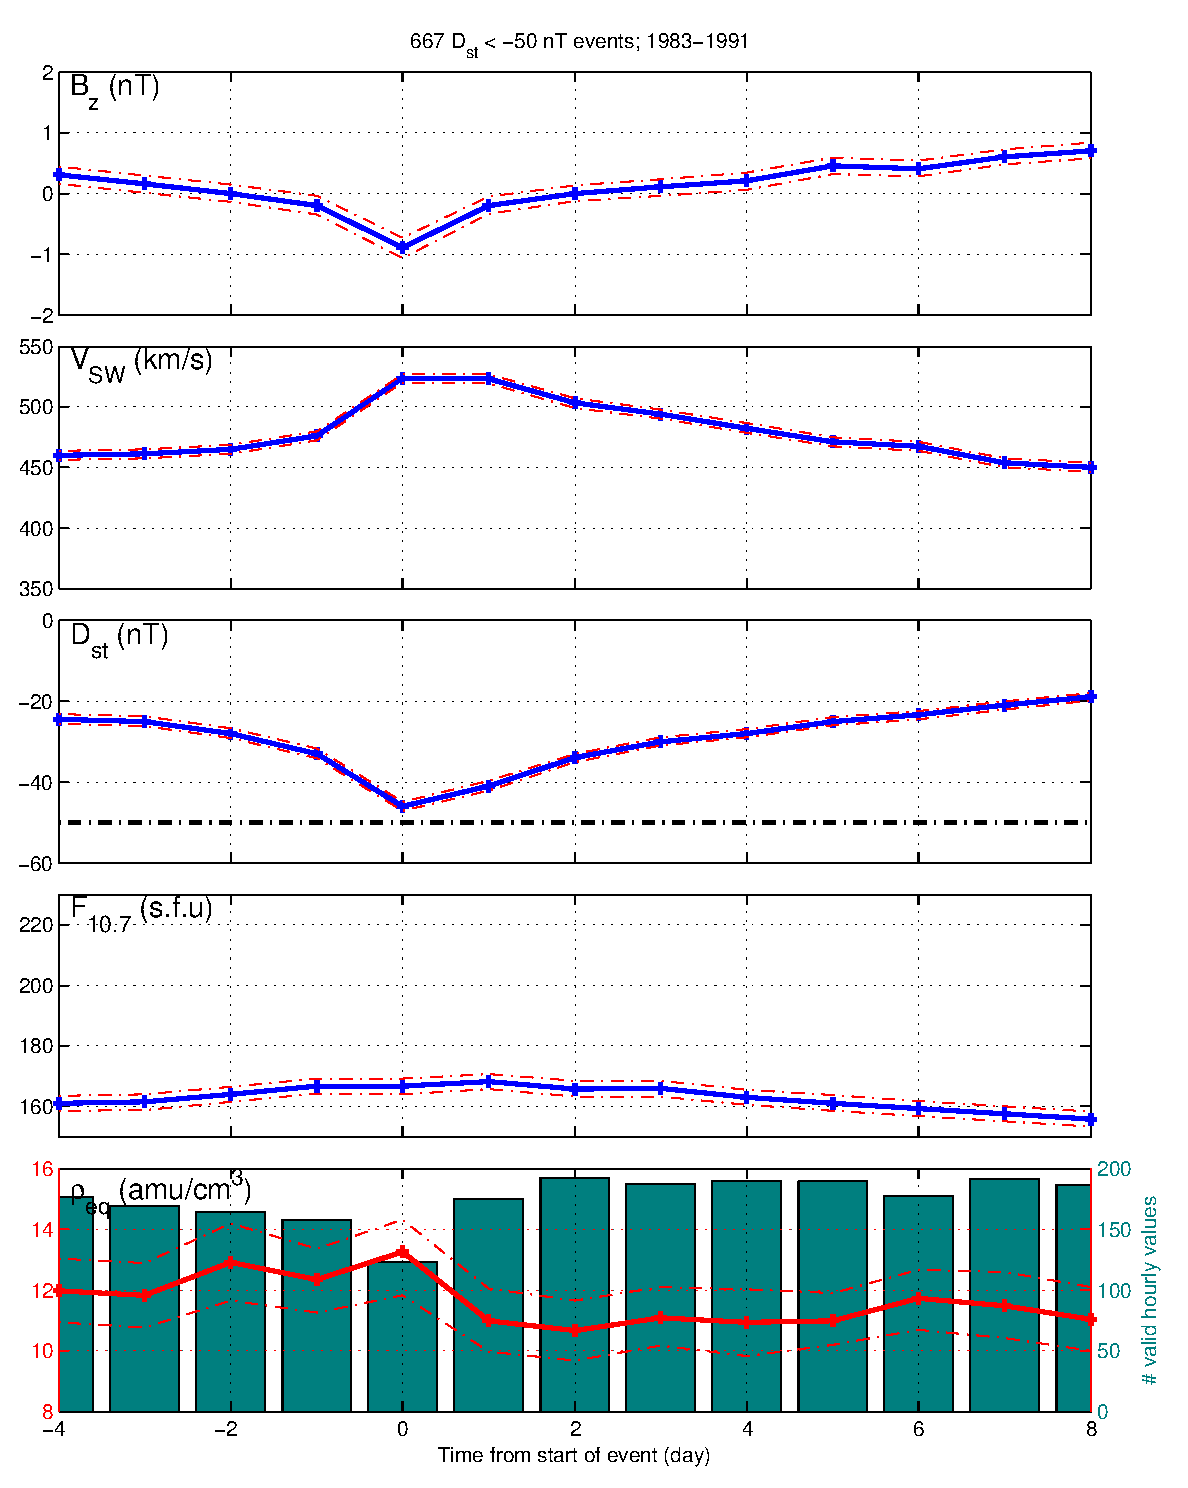
\includegraphics[width=0.5\linewidth]{Figures/StormAvs/stormavs-dst-day-GOES6}
		\caption{\dst\ events on an hourly (left) and daily (right) timescale.}
		\label{fig:EpochDst}
	\end{figure}
\end{frame}

\begin{frame}
	To verify whether events were significantly different between day of onset and the surrounding days, a bootstrap test of differences was performed:
	\begin{figure}[htp!]
		\centering
		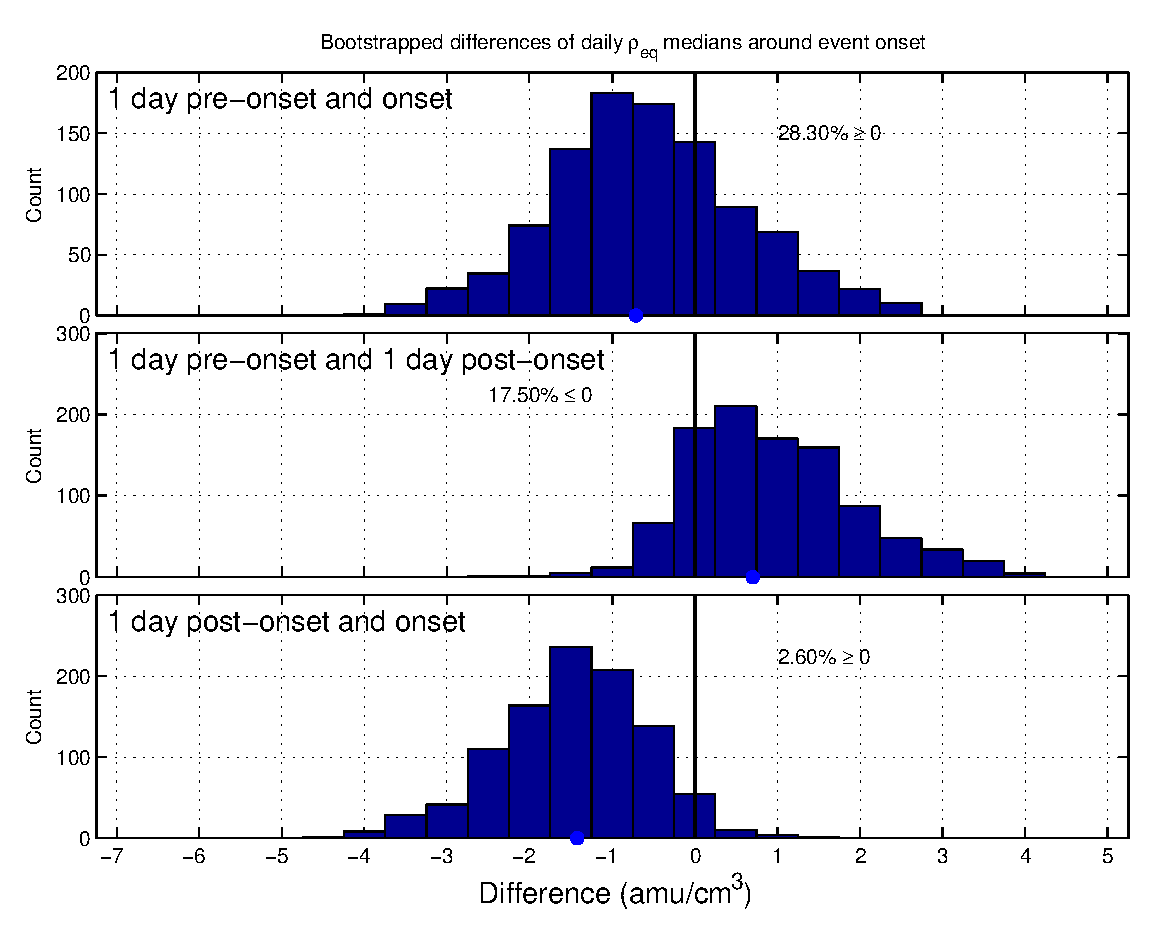
\includegraphics[width=0.6\linewidth]{Figures/DailyBootstrapDifferences-GOES6-case13}
		\caption{Bootstrap differences between median daily value of events using the years of 1983-1991.}
		\label{fig:DailyBootstrapDifferences-full}
	\end{figure}
	
\end{frame}


\begin{frame}
\begin{figure}[htp!]
	\centering
	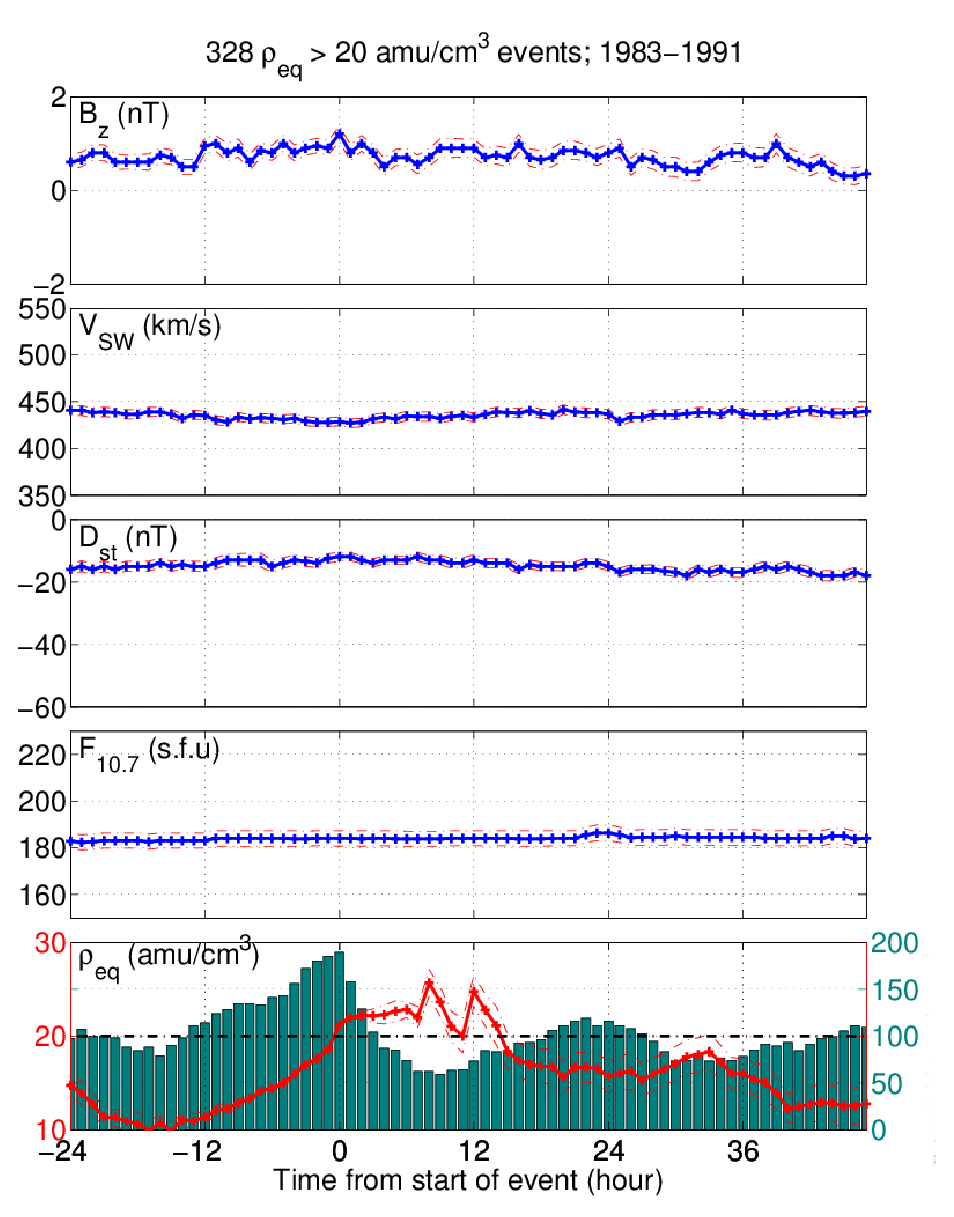
\includegraphics[width=0.4\linewidth]{Figures/StormAvs/stormavs-mass-gt20-GOES6}
	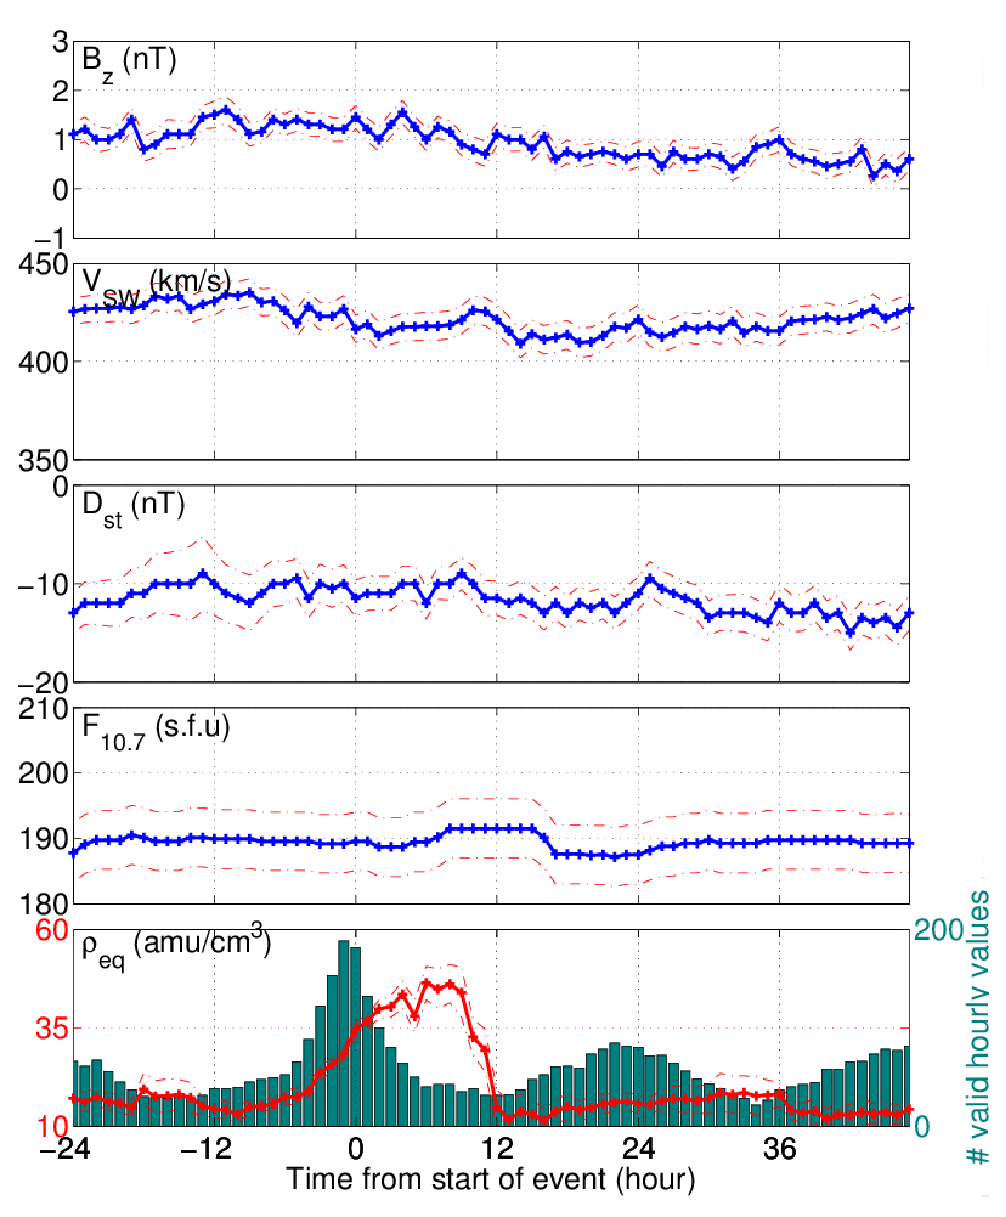
\includegraphics[width=0.4\linewidth]{Figures/StormAvs/stormavs-diffden-5amu-GOES6}
	\caption{Left: \req\ events on hourly timescale. Right: \req\ events where \req\ increased by at least 5 amu during onset hour. Daily averages showed similar lack of significance and median northward $B_z$.}
	\label{fig:EpochDst12Hour}
\end{figure}
\end{frame}


\begin{frame}
	Want to investigate nonlinear dependencies by binning events:
	\begin{figure}[htp!]
		\centering
		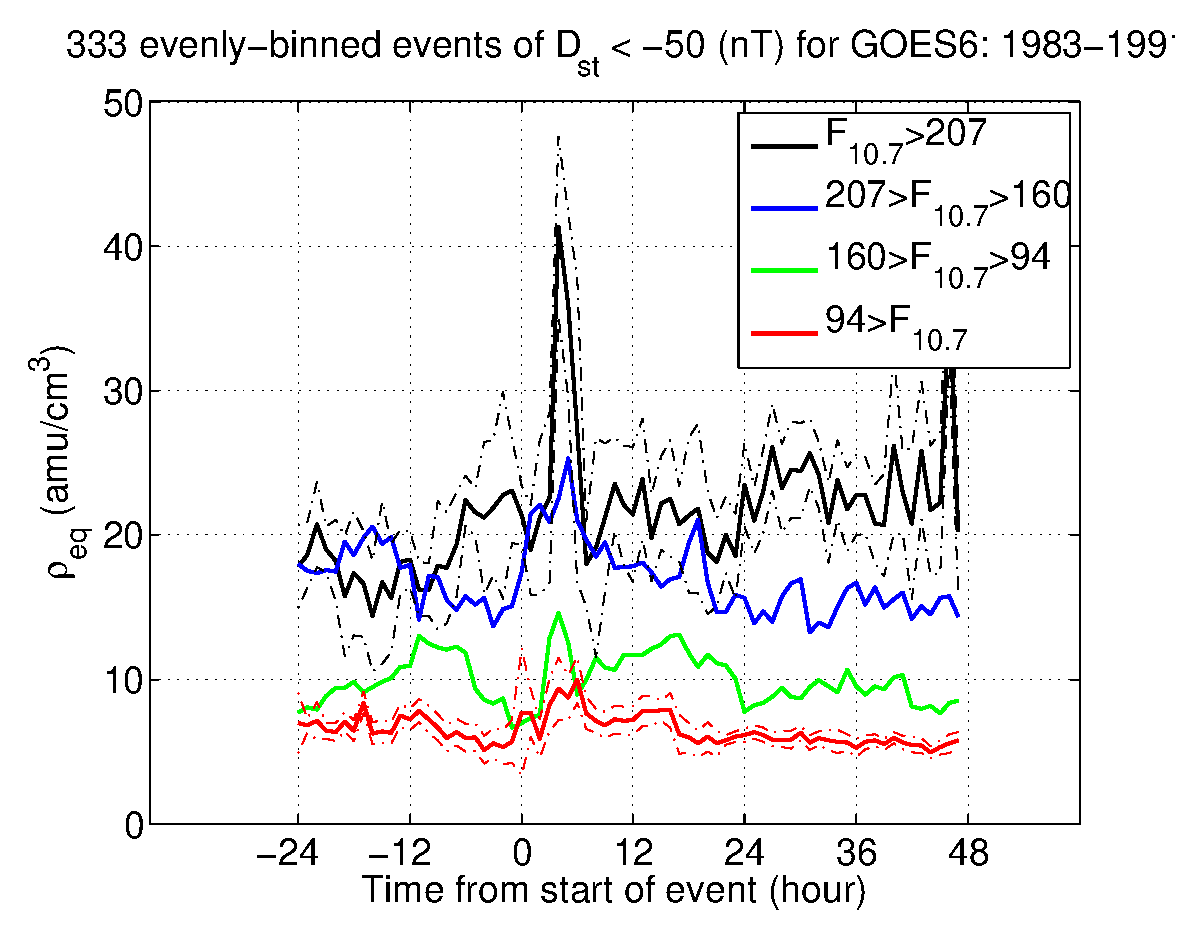
\includegraphics[width=0.5\linewidth]{Figures/HighLowF107rhoeq-Dst50-GOES6-1983-1991}
		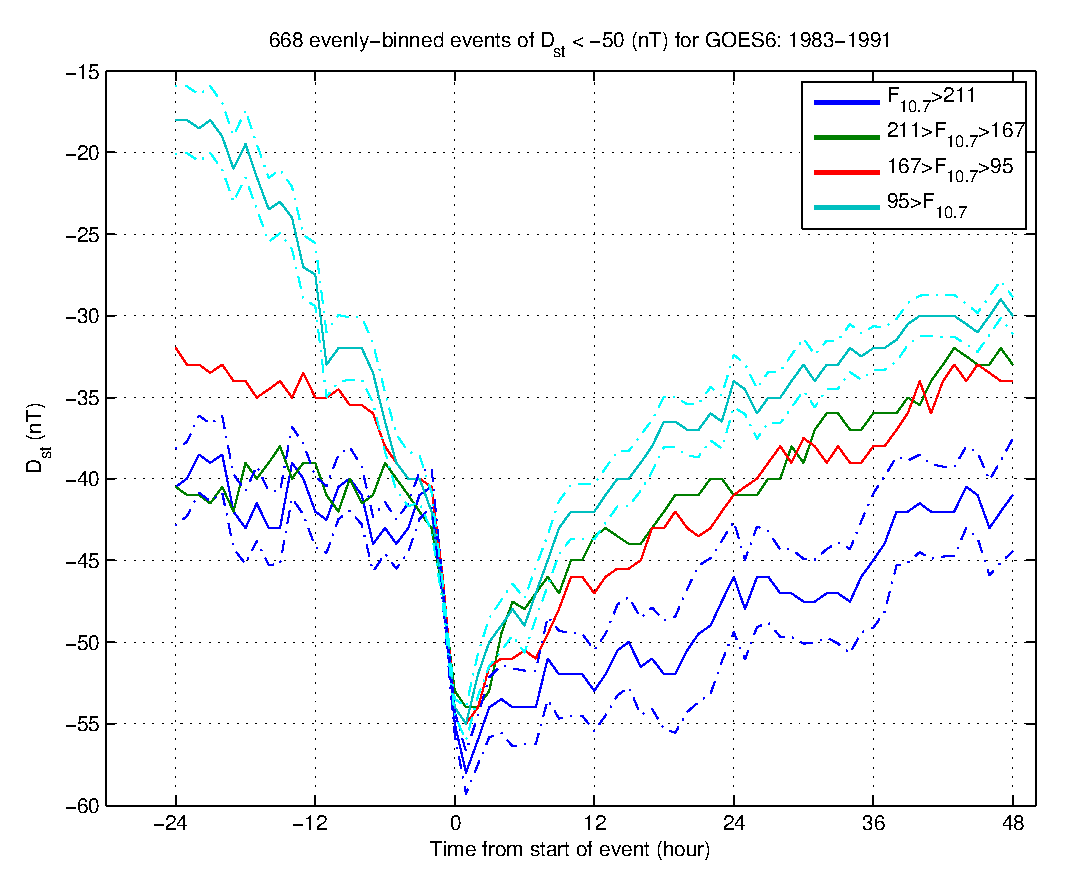
\includegraphics[width=0.5\linewidth]{Figures/HighLowF107Dst-Dst50-GOES6-1983-1991}	
		\caption{\req\ (left) and \dst\ (right) of \dst\ events binned by median \f\ values.}
		\label{fig:HighLowF107rhoeq}
	\end{figure}
\end{frame}

\begin{frame}
	Verifying that distribution of \req\ is significantly different per \f\ bin before \req\ or \dst\ event onset.
	\begin{figure}[htp!]
		\centering
		\includegraphics[width=0.5\linewidth]{Figures/RhoBinnedF_{10.7}-case24-t020-tf25-GOES6}
		\includegraphics[width=0.5\linewidth]{Figures/RhoBinnedF_{10.7}-case1-t020-tf25-GOES6}
		\caption{\req\ events (left) and \dst\ events (right) binned by median \f\ before event onset.}
		\label{fig:RhoBinnedF107}
	\end{figure}
\end{frame}

\begin{frame}
	Attempting to bin by IMF following event:
		\begin{figure}[htp!]
			\centering
			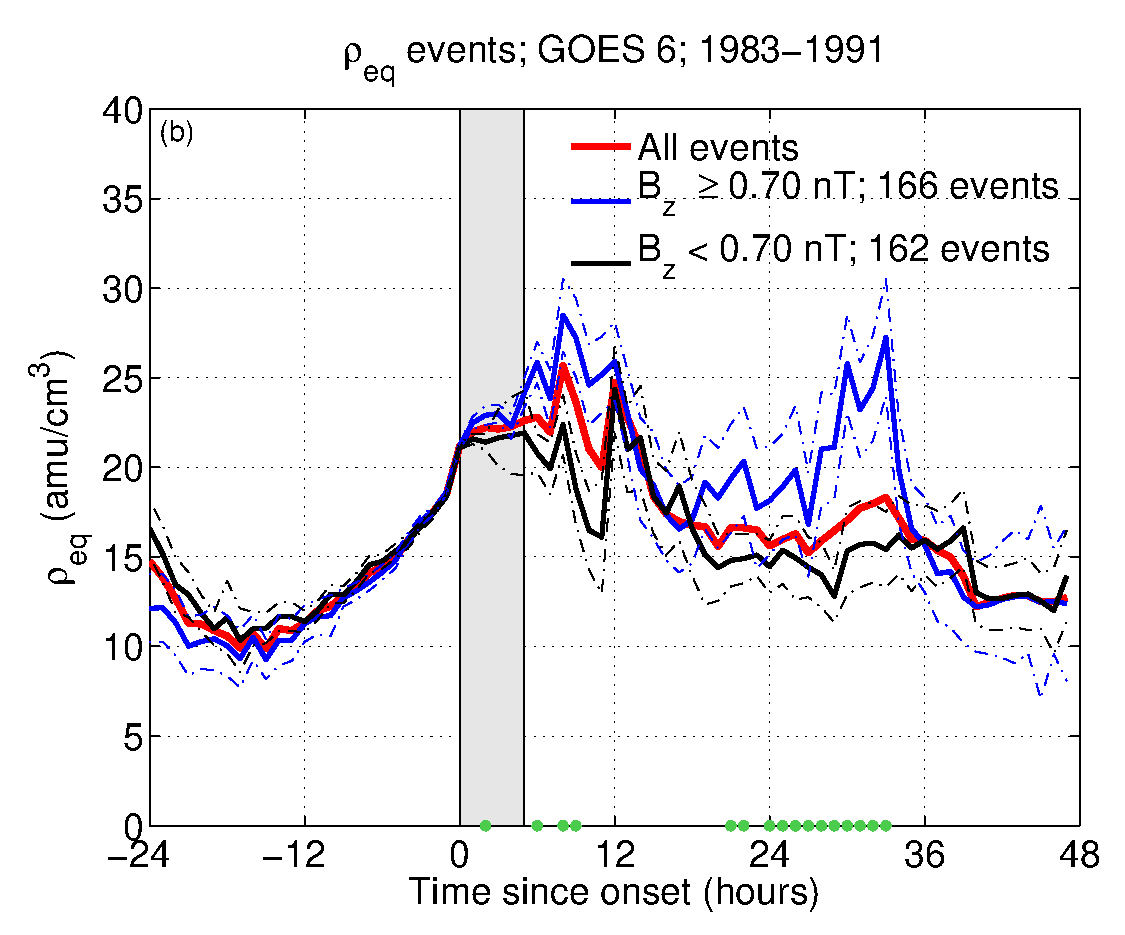
\includegraphics[width=0.5\linewidth]{Figures/RhoBinnedB_z-case24-t025-tf30-GOES6}
			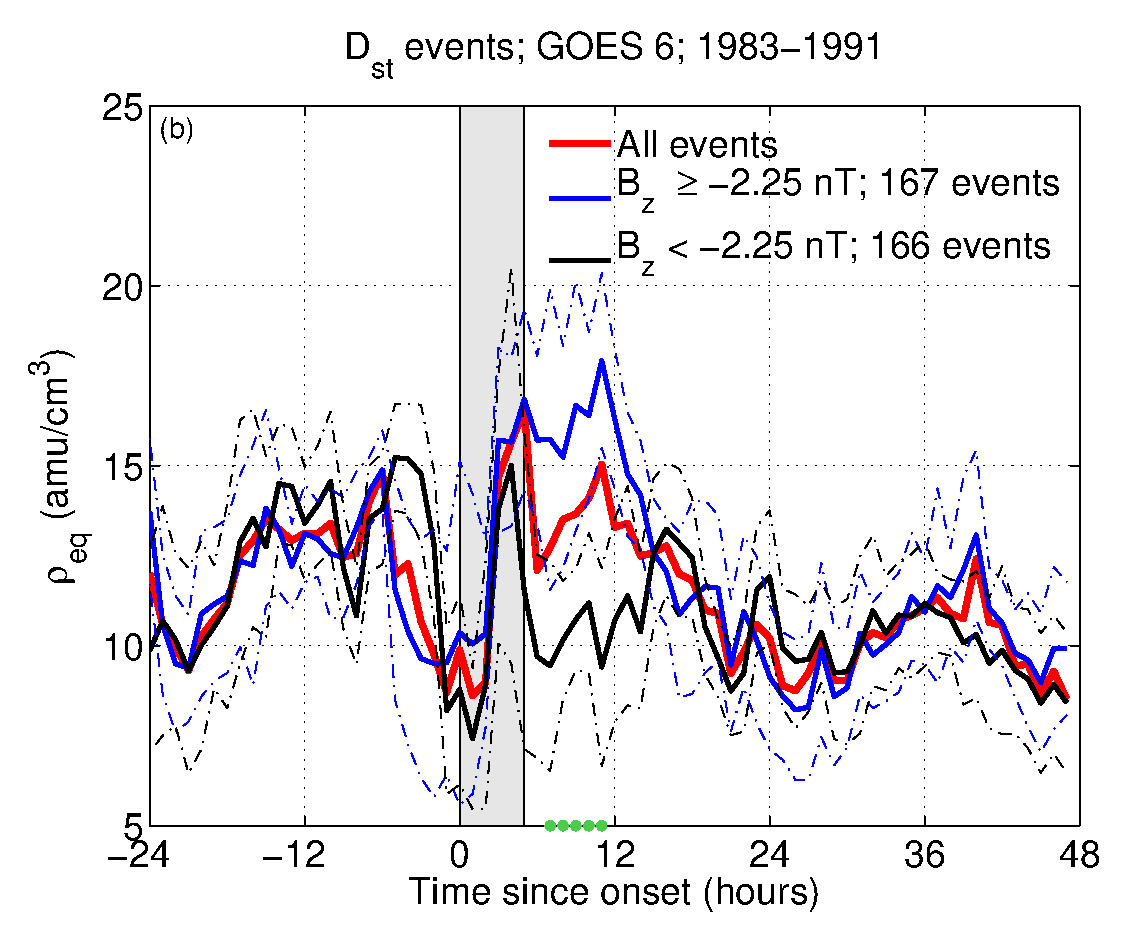
\includegraphics[width=0.5\linewidth]{Figures/RhoBinnedB_z-case1-t025-tf30-GOES6}
			\caption{\req\ events (left) and \dst\ events (right) binned by median $B_z$ after event onset.}
			\label{fig:RhoBinnedF107}
		\end{figure}
\end{frame}

\begin{frame}
	Can conclude:
	\begin{itemize}
		\item \req\ decreases significantly between the day of a \dst\ event and the day following
		\item Elevated \f\ coincides with elevated \req\ before and after \req\ events
		\item Elevated \f\ enables a short, multi-hour spike in \req\ following a \dst\ event
		\item Northward IMF at \req\ event onset supports elevated \req\ over following 36 hours
	\end{itemize}
\end{frame}

\subsection{Classification and Forecasting}
\begin{frame}
	\subheader
	Two main questions:
	\begin{itemize}
		\item Can \req\ event onset criteria be determined by current IMF and geomagnetic conditions?
		\item Can event onsets be forecasted using the hours or days before?
	\end{itemize}
	\vspace{1em}
	Utilizing MATLAB's \texttt{patternnet} neural network toolbox, classifying onsets as ``1" and all other times as ``0". Weighting ``1"s more heavily based on timescale since events are much less frequent than non-events.
\end{frame}


\begin{frame}
	Classifying \req\ events using \f, Kp, \dst, and $V_{SW}$ finds:
	\begin{itemize}
		\item Hourly averaged data: 19\% positive identification accuracy\\
		\item Daily averaged data: 70\% positive identification accuracy\\
		\item Equal distribution of values for correct and incorrect classifications
	\end{itemize}
	
		\begin{figure}[htp!]
			\centering
			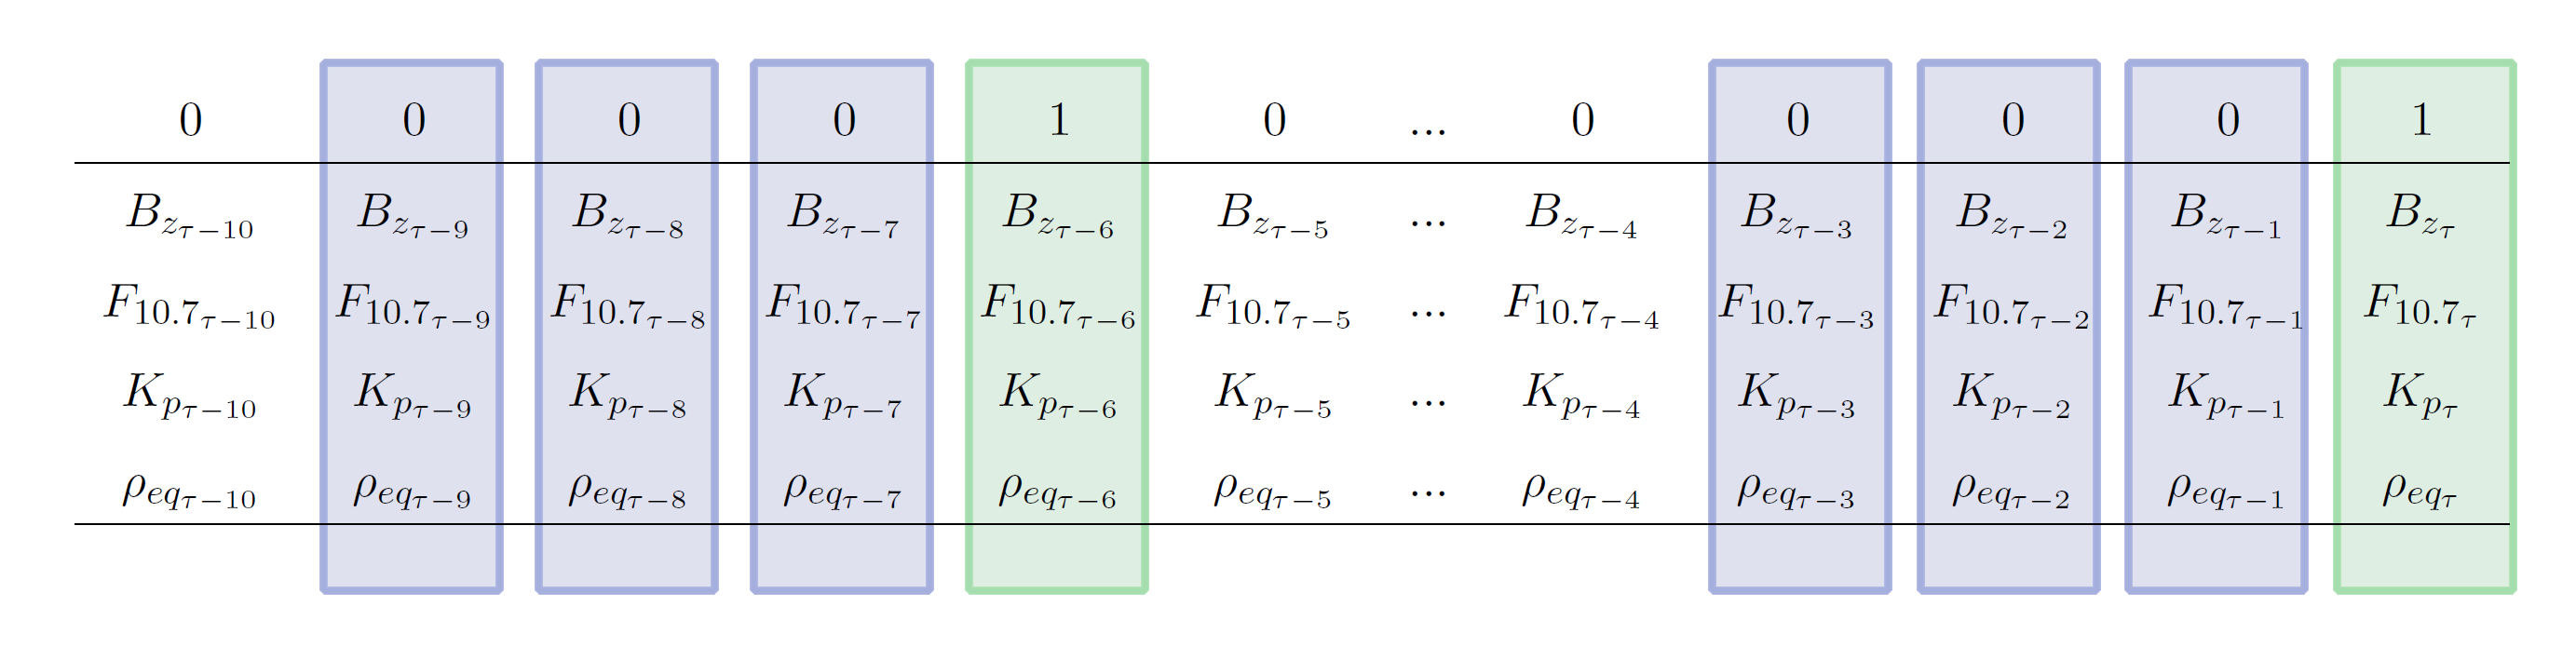
\includegraphics[width=1\linewidth]{Figures/CH5/ClassifyGraphic-2.png}
		\end{figure}
\end{frame}

\begin{frame}
	Predicting \req\ onsets using \f, Kp, \dst, $V_{SW}$, and \req finds:
	\begin{itemize}
		\item Hourly averaged data: 0\% positive prediction accuracy (12k+ predictions, 140 events)\\
		\item Daily averaged data: 58\% positive prediction accuracy\\
		\item Low daily \f\ leads to false negatives suggesting high \f\ better indicator of event
	\end{itemize}
	
		\begin{figure}[htp!]
			\centering
			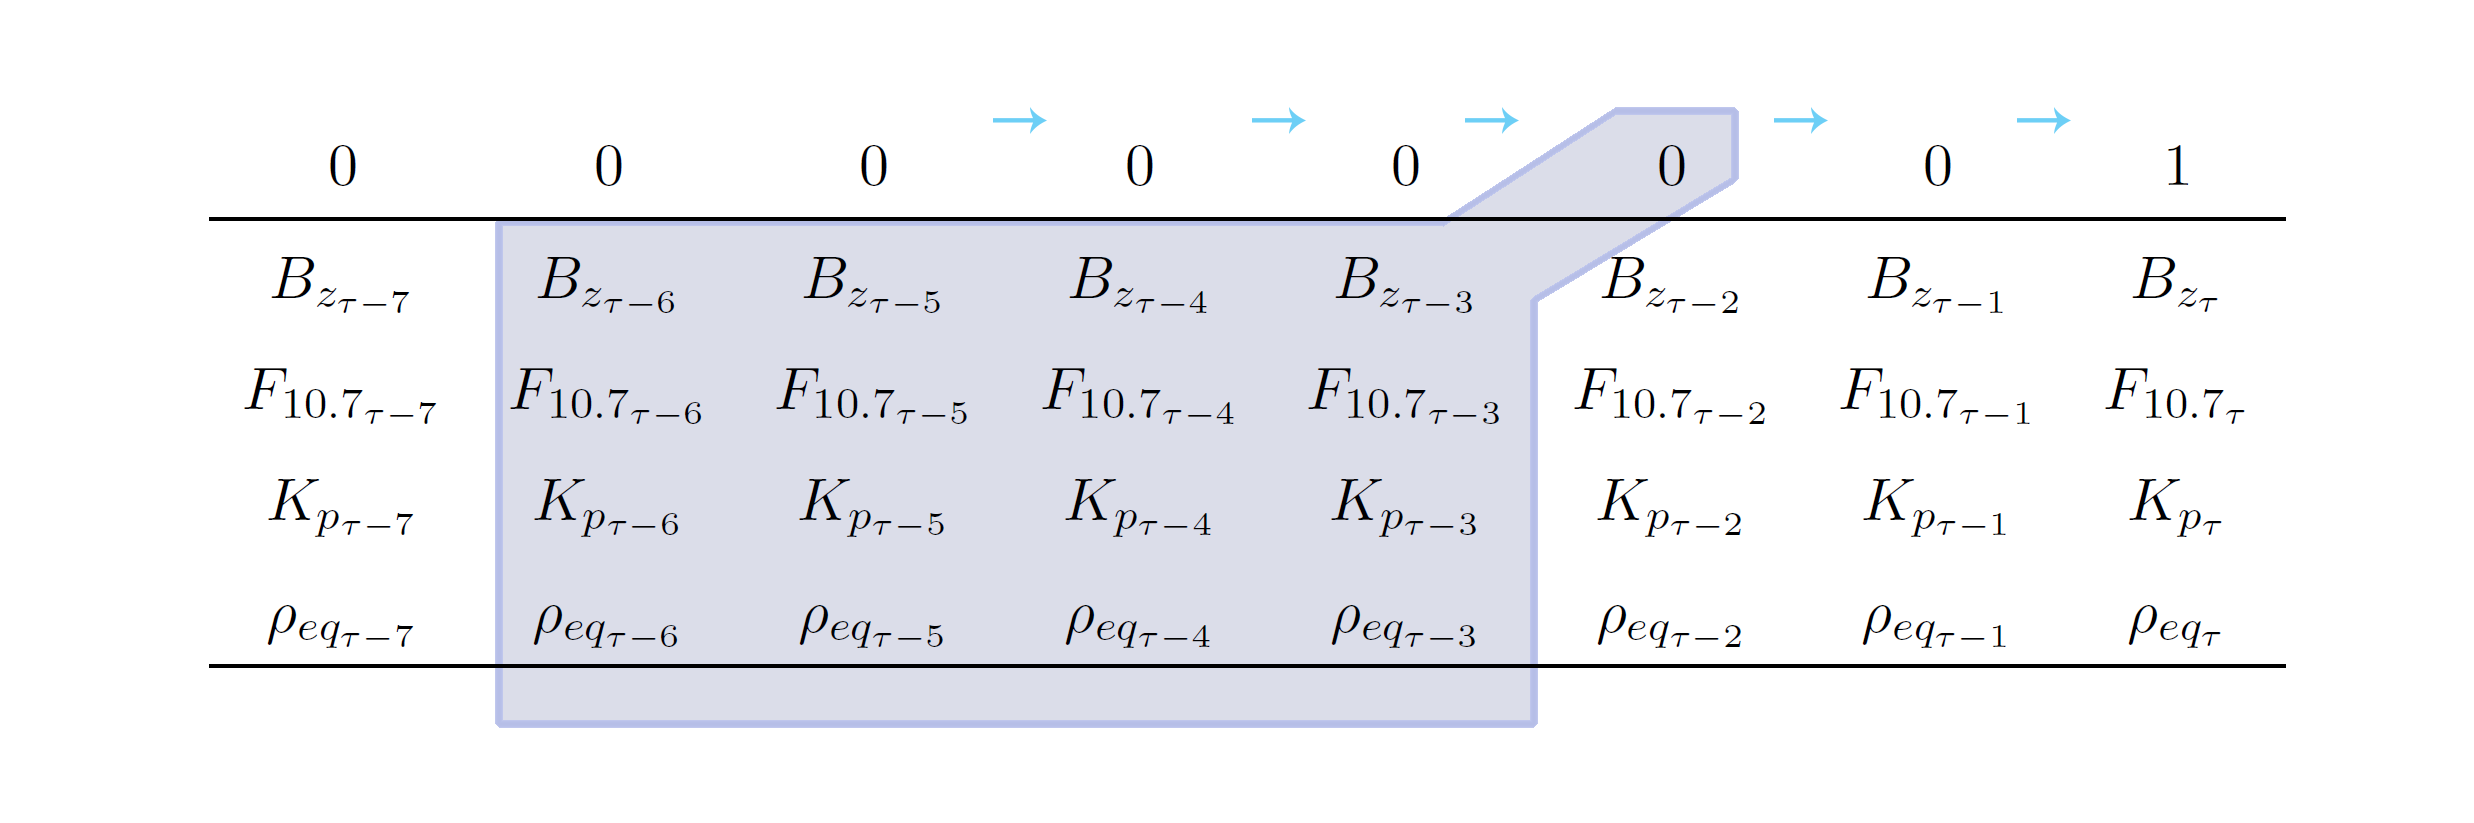
\includegraphics[width=1\linewidth]{Figures/CH5/FullGraphic-2.png}
		\end{figure}
\end{frame}



%%%%%%%%%%%%%%%%%%%%%%%%%%%%%%%%%%%%%%%%%%%%%%%%%%%
%  _____                  _           _                 
% /  __ \                | |         (_)                
% | /  \/ ___  _ __   ___| |_   _ ___ _  ___  _ __  ___ 
% | |    / _ \| '_ \ / __| | | | / __| |/ _ \| '_ \/ __|
% | \__/| (_) | | | | (__| | |_| \__ | | (_) | | | \__ \
% \_____/\___/|_| |_|\___|_|\__,_|___|_|\___/|_| |_|___/
%%%%%%%%%%%%%%%%%%%%%%%%%%%%%%%%%%%%%%%%%%%%%%%%%%%
\section{Conclusions}
\subsection{Conclusions}
\begin{frame}
	To reitterate the initial questions:	
	\begin{itemize}
		\item What enhances \req\ in the plasmatrough? Solar wind (via geomagnetic storms) or internal processes (e.g. ionospheric outflow)?
		\item[] \textbf{Geomagnetic storms not nearly as impactful as internal processes, such as outflow driven by \f, and processes enabled by high \f.}
		\item Does a \req\ enhancement depend on current IMF conditions?
		\item[] \textbf{Weakly. Northward IMF supports higher \req\ after either type of event.}
		\item Can a \req\ enhancement be classified or forecasted?
		\item[] \textbf{Not well using most common solar wind and geomagnetic variables. Suggests something else needed.}
	\end{itemize}
\end{frame}

\begin{frame}
	Further conclusions:
	\begin{itemize}
		\item Drop in \dst\ does not significantly influence \req\ on an hourly timescale, but does over the following day.
		\item \req\ increases do not correlate, on average, with significant changes in \dst, \f, or $B_z$.
		\item Classifying or forecasting the day of an event onset are possible but both prone to false positives or false negatives, depending on weighting.
	\end{itemize}
\end{frame}


\subsection{Future work}
\begin{frame}
	\subheader
	\begin{itemize}
		\item Exploring remaining signal after all collinear variables removed
		\item Adding model complexity and extra information
		\item Use new satellites and/or new Alfvén wave detection methods
		\item Extend time period of analysis
	\end{itemize}
\end{frame}


\begin{frame}[c]
	\begin{center}
		\huge
		\begin{beamercolorbox}[sep=18pt,center,shadow=true,rounded=true]{title}
			\usebeamerfont{title}Thank you for your time.\par%
		\end{beamercolorbox}
		\vspace{2em}
		Questions?
	\end{center}

\end{frame}







\end{document}